\documentclass[cn,table]{elegantbook}

\usepackage{tikz}
\usepackage{graphicx}
\usepackage{subcaption}
\usepackage[ruled,linesnumbered,vlined]{algorithm2e}
\usepackage{hyperref}
\usepackage{listings}
\usepackage{interval}
\usepackage{xcolor}
\usepackage{ulem}
\usepackage{wrapfig}

\intervalconfig{%
	soft open fences,
}

\def\figureautorefname{图}
\def\sectionautorefname{小节}

\SetAlgorithmName{算法}{算法}{算法索引}

\renewcommand*{\lstlistingname}{代码}

\title{何老师算法课笔记}
\subtitle{Always be patient, sharp and diligent.}
\author{计卓1801全体}
\institute{华中科技大学}
\date{\zhtoday}
\version{1.8.0}
\logo{logo.png}
\cover{cover.png}

\begin{document}
\maketitle
\tableofcontents
\pagenumbering{arabic}

% add your code here
% \chapter{Example}

\begin{introduction}
	\item 提要1
	\item 提要2
	\item 提要3
	\item 提要4
	\item 提要5
\end{introduction}

这是一个示例。

\section{环境}

\begin{theorem}{xxx定理}{label-for-this-theorem}
	这是一个定理。
\end{theorem}

\begin{example}
	这是一个例题。
\end{example}

\begin{definition}{xxx}{label-for-this-def}
	这是一个定义。
\end{definition}

\begin{lemma}{xxx引理}{label-for-this-lemma}
	这是一个引理。
\end{lemma}

\begin{proposition}{xxx命题}{label-for-this-prop}
	这是一个命题。
\end{proposition}

这是一个列表:

\begin{itemize}
	\item first thing
	\item second thing
	      \begin{itemize}
		      \item more of second thing
	      \end{itemize}
	\item third thing
	      \begin{enumerate}
		      \item 可以是有序列表
		      \item more of enumerate
	      \end{enumerate}
\end{itemize}

这是一张图片:

\begin{figure}[hbt]
	\centering
	\includegraphics{image/dynamic-programming-1.png}
	\caption{这是一张图片}\label{fig:example}
\end{figure}

这是一段代码:

\begin{lstlisting}[language=Python, caption=Python example]
import numpy as np

def incmatrix(genl1,genl2):
    m = len(genl1)
    n = len(genl2)
    M = None #to become the incidence matrix
    VT = np.zeros((n*m,1), int)  #dummy variable

    #compute the bitwise xor matrix
    M1 = bitxormatrix(genl1)
    M2 = np.triu(bitxormatrix(genl2),1)

    for i in range(m-1):
        for j in range(i+1, m):
            [r,c] = np.where(M2 == M1[i,j])
            for k in range(len(r)):
                VT[(i)*n + r[k]] = 1;
                VT[(i)*n + c[k]] = 1;
                VT[(j)*n + r[k]] = 1;
                VT[(j)*n + c[k]] = 1;

                if M is None:
                    M = np.copy(VT)
                else:
                    M = np.concatenate((M, VT), 1)

                VT = np.zeros((n*m,1), int)

    return M
\end{lstlisting}

更多环境请见文档。

\section{引用}

\subsection{交叉引用}

引用定理~\ref{thm:label-for-this-theorem}。

\subsection{参考文献}

引用一个参考文献~\cite{cormen2009introduction}

\chapter{算法渐进分析}

\begin{introduction}
	\item 渐进记号
	\item 渐进增长的性质
	\item 常见的渐进函数
\end{introduction}

\section{关于算法的计算效率}
当我们在了解计算效率或者研究算法的复杂度时,我们主要集中于运行算法的时间效率
--因为我们总是希望能够更快地运行算法。当然对于空间复杂度也是不能够忽略的,
不过一下我们主要以算法的时间复杂度为载体,介绍算法的渐进分析,空间复杂度的分析
可以进行类比。

一个算法在规模为n的输入下,最坏情况运行时间增长率最多与某个函数$f(n)$成正比,
函数$f(n)$因此就成为了我们算法运行时间的一个界限,下面将对此进行详细讨论。

\section{\texorpdfstring{$O,\ \Omega,\ and\ \Theta $}{O, Ω, and θ}}
在这里,我们希望寻找一种表达算法时间复杂或者是其他函数的方法,在这种方法中,常数系数和低次项
对结果是没有影响的。比如 $1.62n^2+3.5n+2.3$ 增长的方式和 $n^2$ 一样。

\begin{figure}[h]
	\begin{minipage}[t]{1\linewidth}
		\centering
		\includegraphics[width=10cm,height=3.5cm]{image/asymptotic_analysis_1.png}
		\caption{$O,\ \Omega,\ and\ \Theta $}
	\end{minipage}
\end{figure}

\subsection{渐进上界 $O$}
令 $f(n)$ 为算法在输入规模为n的情况下的运行时间 (最坏情况),给定另一个函数 $g(n)$,当n充分大,
函数 $f(n)$ 不会超过 $g(n)$ 的常数倍,就有 $f(n)=O(g(n))$。数学定义如下:

\begin{definition}{O ($\cdot$)}{def1}
	\[
		O(g(n))= \{f(n): \exists\ c,n_0\in R^+,such\ that: \forall n\ge n_0:0\le f(n)\le cg(n)\}
	\]
\end{definition}


举个例子作为说明,假设算法的运行时间有着$f(n)=pn^2+qn+r$的形式,其中p,q,r均为正常数,我们可以说
任何具有这种形式的函数都是$O(n^2)$即$pn^2+qn+r=O(n^2)$ ,证明如下:
\begin{proof}
	\begin{align*}
		\forall n \geq 1,t     & hen\ qn\leq qn^2,r\leq rn^2 \\
		\Longrightarrow   f(n) & =pn^2+qn+r                  \\
		                       & \leq pn^2+pn^2+rn^2         \\
		                       & =(p+q+r)n^2
	\end{align*}
\end{proof}
注意到$O(\cdot)$仅仅代表一个上界,并不代表函数准确的增长率,例如$pn^2+qn+r=O(n^3)$也是成立的
但是它不是“最紧”的一个上界。
\subsection{渐进下界\ $\Omega$}
对于算法的渐进下界,我们同样可以对其进行说明:令$f(n)$为算法在输入规模为n的情况下的运行时间,给
定另一个函数$g(n)$,如果对充分大的n,函数$f(n)$至少是函数$g(n)$的常数倍,就有$f(n)=\Omega(g(n))$
\begin{definition}{$\Omega(\cdot)$}{def2}
	\[
		\Omega (g(n))= \{f(n): \exists\ c,n_0\in R^+,such\ that: \forall n\ge n_0:0\le cg(n)\le f(n)\}
	\]
\end{definition}

继续使用 $f(n)=pn^2+qn+r$ 的例子,其中q 、p、 r 均为正常数,我们可以说具有任何这种形式的函数都是$\Omega(n)$。
证明如下:
\begin{proof}
	\begin{align*}
		\forall n \geq 1,t     & hen\ qn\leq 0,r\geq 0 \\
		\Longrightarrow   f(n) & =pn^2+qn+r            \\
		                       & \geq pn^2+pn^2+rn^2   \\
		                       & =(p+q+r)n^2
	\end{align*}
\end{proof}

同$O(\cdot)$的情况,我们注意到$\Omega(\cdot)$仅仅代表一个下界,例如:$f(n)=pn^2+qn+r=\Omega(n)$也是成立的。

\subsection{渐进紧界$\Theta$}
在上面知识的支持下,我们发现,对于同一个$f(n)$,其上下界,所对应的$g(n)$可能是相同的,即$f(n)=O(g(n))$并且$f(n)=\Omega(g(n))$
,在这种情况下,我们可以说$f(n)=\Theta(g(n))$
\begin{definition}{$\Theta(\cdot)$}{def3}
	\[
		\Theta(g(n)) = \{f(n): \exists\ c_1,c_2,n_0\in R^+,such\ that: \forall n\ge n_0:0\le c_1 g(n)\le f(n)\le c_2 g(n)\}
	\]
\end{definition}

沿用刚才的例子,对于$f(n)=pn^2+qn+r$,我们可以说任何具有该
形式的函数都是$\Theta(n^2)$的,对于其证明就再简单不过了,我们只需要将上面两段合起来即可!
在实际的计算中,对于显示的函数,我们为了求得$\Theta(\cdot)$,只需保留其最大幂的多项式或者主要成分,去掉常数项即可。
\\
\\
除了刚刚介绍的方法,我们还可以利用以下性质求得$\Theta(\cdot)$:
\\
设$f$和$g$是两个函数,并且
\[
	\lim_{n\rightarrow+\infty}\frac{f(n)}{g(n)} = c \ (c\ge 0)
\]
那么$f(n)=\Theta(g(n))$,关于该部分的证明,留给读者自行探索。


\section{渐进增长的一些性质}
下面将给出渐进增长的一些性质,对于性质的证明,可以自己证明,然后与\cite{textbook1}的P38-P40的证明进行对照
\begin{theorem}{Transitivity}{}
	(a)\ If\ $f=O(h)$\ and\ $g=O(h)$, then $f=O(h)$\\
	(b)\ If\ $f=\Omega(h)$\ and\ $g=\Omega(h)$, then $f=\Omega(h)$\\
	(c)\ If\ $f=\Theta(h)$\ and\ $g=\Theta(h)$, then $f=\Theta(h)$
\end{theorem}

\begin{theorem}{Sum\ of\ Functions}{}
	假设$f$和$g$是两个函数,若对某个其他的函数$h$,都有:$f=O(h),g=O(h)$\\
	那么,$f+g=O(h)$\\
	推广开来:令k是确定的常数,$f_1,f_2,f_3,\ldots,f_k$和$h$是函数,且
	$f_i=O(h)$ \ \ $i\in (1,k)$,\\
	那么,$\sum^{k}_{i=1}f_i=O(h)$
\end{theorem}

\begin{theorem}{}{}
	假设 $f$ 和 $g$ 是两个函数, (取非负值),使得 $g = O(f)$ \\
	那么 $f+g=\Theta(f)$
\end{theorem}

\section{常见的渐进函数}
在一般的算法复杂度的分析中,我们常使用$O(\cdot)$进行渐进分析,其中常用的函数有以下几个:\\
算数级复杂度:
\[
	O(1)<O(logn)<O(n)<O(nlogn)<O(n^2)<O(n^2logn)<O(n^3)< \cdots
\]

指数级复杂度:
\[
	O(2^n)<O(n!)<O(n^n)
\]

如要了解更多的标准记号和常用函数,可以参考~\cite{cormen2009introduction}

\chapter{骨牌问题 (Tiling Problem)}

\begin{introduction}
    \item 定义
    \item 形状为$2\times1$的骨牌
\end{introduction}

\section{问题定义}\label{sec:tiling-1}
\begin{definition}{骨牌问题}{def:tiling-problem}
    给出大小确定数量不限的骨牌,问能否不重叠的铺满整个平面
\end{definition}

\section{骨牌形状为\texorpdfstring{$2\times1$}{}}\label{sec:tiling-2}
    骨牌形状为$2\times1$(如\autoref{fig:tiling-1}),判断使用该种骨牌能不能不重叠的铺满给定的平面。
    形状为$2\times1$的骨牌的填充问题属于$P$类问题。
    下面是一些用这种骨牌填充的例题。
    \begin{figure}[hbt!]
        \centering
        \begin{tabular}{|c|}
            \hline
            \\ \hline
            \\ \hline
        \end{tabular}
        \caption{形状为$2\times1$的骨牌}
        \label{fig:tiling-1}
    \end{figure}
\subsection{形状为\texorpdfstring{$M\times N$}{}的矩形}\label{subsec:tiling-2-1}
    这种完整的矩形(如\autoref{fig:tiling-2})是简单问题。只需要判断形状中的格子数目($M\times N$)是否为偶数。
    如果格子的数目为偶数,则能填满。
    如果格子的数目为奇数则不能填满。
    \begin{figure}[hbt!]
        \centering
        \begin{tabular}{|c|c|c|c@{\dots}c|c|c|c|}
            \cline{1-3} \cline{6-8}
            & & & & & & & \\
            \cline{1-3} \cline{6-8}
            & & & & & & & \\
            \cline{1-3} \cline{6-8}
            \multicolumn{3}{c}{}& &\multicolumn{3}{c}{} \\
            \cline{1-3} \cline{6-8}
            & & & & & & & \\
            \cline{1-3} \cline{6-8}
            & & & & & & & \\
            \cline{1-3} \cline{6-8}
        \end{tabular}
        \caption{$M\times N$的矩形}\label{fig:tiling-2}
    \end{figure}


    如果格子的数目为奇数,显然不能使用$2\times1$的骨牌铺满。而当格子的数目为偶数时,则行或列中必有一个为偶数。显然能用这种骨牌填满。
\subsection{形状为$6\times6$的矩形挖去两个对角}\label{subsec:tiling-2-2}
    \begin{figure}[ht!]
        \begin{subfigure}{0.5\textwidth}
            \centering
            \begin{tabular}{|c|c|c|c|c|c|}
                \cline{2-6}
                \multicolumn{1}{c|}{}& & & & & \\ \hline
                & & & & & \\ \hline
                & & & & & \\ \hline
                & & & & & \\ \hline
                & & & & & \\ \hline
                & & & & &\multicolumn{1}{c}{} \\
                \cline{1-5}
            \end{tabular}
            \caption{挖去两个对角的$6\times6$的矩形}\label{fig:tiling-3}
        \end{subfigure}
        \begin{subfigure}{0.5\textwidth}
            \centering
            \begin{tabular}{|c|c|c|c|c|c|}
                \cline{2-6}
                \multicolumn{1}{c|}{}& \cellcolor[rgb]{0,0,0} & & \cellcolor[rgb]{0,0,0} & & \cellcolor[rgb]{0,0,0} \\ \hline
                 \cellcolor[rgb]{0,0,0} & & \cellcolor[rgb]{0,0,0} & & \cellcolor[rgb]{0,0,0} & \\ \hline
                 & \cellcolor[rgb]{0,0,0} & & \cellcolor[rgb]{0,0,0} & & \cellcolor[rgb]{0,0,0} \\ \hline
                 \cellcolor[rgb]{0,0,0} & & \cellcolor[rgb]{0,0,0} & & \cellcolor[rgb]{0,0,0} & \\ \hline
                 & \cellcolor[rgb]{0,0,0} & & \cellcolor[rgb]{0,0,0} & & \cellcolor[rgb]{0,0,0} \\ \hline
                 \cellcolor[rgb]{0,0,0} & & \cellcolor[rgb]{0,0,0} & & \cellcolor[rgb]{0,0,0} &\multicolumn{1}{c}{} \\
                \cline{1-5}
            \end{tabular}
            \caption{染色后的矩形}\label{fig:tiling-4}
        \end{subfigure}
        \caption{}
    \end{figure}
    这种情况下(如\autoref{fig:tiling-3}),格子的总数为34个,是个偶数。所以可以尝试通过对格子进行染色的方式判断。选取其中一个格子染成和黑色,
    对黑色上下左右相邻的格子染成白色,对白色上下左右相邻的格子染成黑色(结果如\autoref{fig:tiling-4})。染色是判断能否被填充的一个方法。
    这种方法得到的不可填充的结论是可信的,但可填充的结论却不一定可信。

    统计黑色和白色格子的数目,黑色有18个,白色有16个。而将骨牌染成黑白两色,发现需要被填充的形状中黑色和白色的个数不同。所以这种形状无法被$2\times1$的骨牌填充。
\subsection{一个奇异的形状}\label{subsec:tiling-2-3}
    \begin{figure}[h!]
        \begin{subfigure}{0.5\textwidth}
            \centering
            \begin{tabular}{|c|c|c|c|c|c|c|c|c|c|}
                \cline{2-4} \cline{7-9}
                \multicolumn{1}{c|}{} & & & & \multicolumn{1}{c}{} & \multicolumn{1}{c|}{} & & & & \multicolumn{1}{c}{} \\ \hline
                 & & & & & & & & & \\ \hline
                 & & & & & & & & & \\ \hline
                 & & & & & & & & & \\ \hline
                \multicolumn{1}{c|}{} & & & & \multicolumn{1}{c}{} & \multicolumn{1}{c|}{} & & & & \multicolumn{1}{c}{} \\
                \cline{2-4} \cline{7-9}
            \end{tabular}
            \caption{一个例子}\label{fig:tiling-5}
        \end{subfigure}
        \begin{subfigure}{0.5\textwidth}
            \centering
            \begin{tabular}{|c|c|c|c|c|c|c|c|c|c|}
                \multicolumn{5}{c!{\color[rgb]{1,0,0}\vline}}{} & \multicolumn{5}{c}{} \\
                \cline{2-4} \cline{7-9}
                \multicolumn{1}{c|}{} & \cellcolor[rgb]{0,0,0} & & \cellcolor[rgb]{0,0,0} & \multicolumn{1}{c!{\color[rgb]{1,0,0}\vline}}{} & \multicolumn{1}{c|}{} & & \cellcolor[rgb]{0,0,0} & & \multicolumn{1}{c}{} \\ \hline
                 \cellcolor[rgb]{0,0,0} & & \cellcolor[rgb]{0,0,0} & & \multicolumn{1}{c!{\color[rgb]{1,0,0}\vline}}{\cellcolor[rgb]{0,0,0}}  & & \cellcolor[rgb]{0,0,0} & & \cellcolor[rgb]{0,0,0} & \\ \hline
                 & \cellcolor[rgb]{0,0,0} & & \cellcolor[rgb]{0,0,0} & \multicolumn{1}{c!{\color[rgb]{1,0,0}\vline}}{} & \cellcolor[rgb]{0,0,0} & & \cellcolor[rgb]{0,0,0} & & \cellcolor[rgb]{0,0,0} \\ \hline
                 \cellcolor[rgb]{0,0,0} & & \cellcolor[rgb]{0,0,0} & & \multicolumn{1}{c!{\color[rgb]{1,0,0}\vline}}{\cellcolor[rgb]{0,0,0}} & & \cellcolor[rgb]{0,0,0} & & \cellcolor[rgb]{0,0,0} & \\ \hline
                \multicolumn{1}{c|}{} & \cellcolor[rgb]{0,0,0} & & \cellcolor[rgb]{0,0,0} & \multicolumn{1}{c!{\color[rgb]{1,0,0}\vline}}{} & \multicolumn{1}{c|}{} & & \cellcolor[rgb]{0,0,0} & & \multicolumn{1}{c}{} \\
                \cline{2-4} \cline{7-9}
                \multicolumn{5}{c!{\color[rgb]{1,0,0}\vline}}{} & \multicolumn{5}{c}{}
            \end{tabular}
            \caption{染色后}\label{fig:tiling-6}
        \end{subfigure}
    \end{figure}
    在这种情况下(如\autoref{fig:tiling-5}),使用上述方式染色后(如\autoref{fig:tiling-6})发现黑色与白色的块数相同,均为21块。但这个图形却是不可被填充的。

    现假设骨牌能填充这个形状,那么红线左侧和红线右侧都应该是可以被填充满的。但红线左侧的黑色方块比白色方块多4个,需要从右面借4个白色方块才能使左红线侧的褐色方块与白色方块数目相同。
    但红线右侧在不借出黑色方块的情况下最多借出2个白色方块,不满足需求。因此左边是不可能被填满的。所以整个平面也是不可被填满的。

    这个问题还可以用网络流来求解。详见\autoref{sec:network-flows-tiling}。

\chapter{匹配问题(Matching Problem)}

\begin{introduction}
	\item 定义
	\item 算法设计
	\item 算法分析
\end{introduction}

\section{问题引入}\label{sec:stable-matching-def}
现在有n个男性的一个集合$M=\{m_1,\dots,m_n\}$和n个女人性一个集合$W=\{w_1,\dots,w_n\}$。
用$M\times W$来表示$(m,w)$所有可能有序对的一个集合,其中$m\in M,w\in W$。一个匹配(Matching)$S$是一个有序对的集合,
这些有序对来自于$M\times W$,并且每一个来自$M$中的元素和来自$W$中的元素最多在$S$中出现一次。
一个完美匹配(Perfect Matching)$S'$是指每一个来自$M$和$W$中的元素都出现过一次的匹配。
\begin{definition}{匹配(Matching)}{matching}
	对于一个给定的0图$G=(V,E)$,这幅图的一个匹配$M$是图$G$的一个子图(由原来的图的一部分顶点和一部分边构成的图),其中每两条边都不相邻(没有公共顶点)。
	在匹配图中,一个顶点连出的边数至多是一条。如果这个顶点连出一条边,就称这个顶点是已匹配的。$M$中的一条边的两个端点叫做在M中是配对的。
\end{definition}
\begin{definition}{完美匹配(Perfect Matching)}{perfect-matching}
	完美匹配是一个包括了图G中原来的所有顶点的匹配。
\end{definition}
现在我们添加优先级的概念。每一个男性$m\in M$对所有的女性有一个排名。如果在$m$的排名中$w$比$w'$更高,我们说m相对于$w'$更倾向于$w$。
我们把$m$的有序评价叫做他的倾向列表。在$m$的评价中所有人的排名都不相同。类似的,对于每一个$w\in W$也对所有的男性有个排名。

\begin{wrapfigure}[10]{r}{0.25\linewidth}
	\centering
	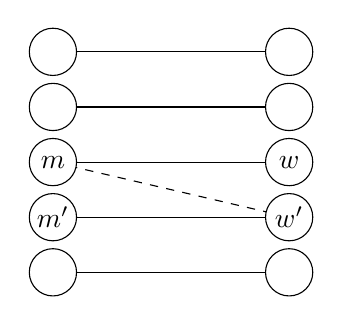
\begin{tikzpicture}
		\draw[dashed] (0,5-0.7*3)  -- (3,5-0.7*4);
		\foreach \x in {5,...,1}
			{
				\draw (0,5-0.7*\x) -- (3,5-0.7*\x);
				\filldraw [fill=white] (0,5-0.7*\x) circle (0.3) node[](m-\x){} (3,5-0.7*\x) circle (0.3) node[](w-\x){};
			}
		\draw
		(m-3) node(){$m$}
		(m-4) node(){$m'$}
		(w-3) node(){$w$}
		(w-4) node(){$w'$};
	\end{tikzpicture}
	\caption{不稳定的情况}
	\label{fig:stable-matching-1}
\end{wrapfigure}
给定一个完美匹配$S$,我们应该担心下面的情况(如\autoref{fig:stable-matching-1})。现在有两个$S$中的匹配$(m,w)$和$(m',w')$,但$m$相对于$w$更倾向于$w'$,
并且$w'$相对于$m'$更倾向于$m$。在这种情况下,没办法阻止$m$和$w'$放弃当前的对象然后组成新的一对。在这种情况下,我们说$(m,w')$对于$S$来说是个不稳定的对。
也就是说,尽管$(m,w')$不存在于$S$中,但$m$和$w'$,相对于他们在$S$中的同伴,更倾向于彼此。

我们的目标是找到一个匹配,这个匹配是完美匹配,并且没有不稳定的对。这个匹配也叫稳定匹配。
\begin{definition}{稳定匹配(Stable Matching)}{stable-matching}
	稳定匹配是一个满足以下条件的匹配:
	\begin{enumerate}[label=(\roman*)]
		\item 是一个完美匹配
		\item 不存在不稳定的的对
	\end{enumerate}
\end{definition}

\section{算法设计}\label{sec:stable-matching-algorithm}
依据上文提到的问题,我们来考虑一下求解方法。
\begin{itemize}[label=$\ast$]
	\item 在最一开始,每个人都是未匹配的。设想一个未匹配的男性$m$选择了在他倾向列表中排名最高的女性$w$,
	      并且提出了请求。所以我们能立刻声明$(m,w)$是我们最后稳定匹配中的一个对吗?不行,在后面有可能$m'$,
	      他在$w$的排名更高,同样向$w$提出了请求。在另一方面,$w$立刻拒绝$m$也是有风险的。她可能不会再收到
	      排名比$m$高的人发出的请求。所以,一个自然地想法是将$(m,w)$对置成约定状态(\sout{约会})。
	\item 假定我们现在处于某个状态,部分是没有匹配的,部分是处于约定状态的。下一步就是一个未匹配的$m$选择了
	      $m$还没有申请过的排名最高的$w$,向$w$提出申请。如果$w$是未匹配的,那么$m$和$w$就成为约定状态。
	      如果$w$是跟$m'$处于约定状态,在这种情况下,$w$根据$m$和$m'$谁的排名更高来选择跟谁成为约定状态,
	      而另一个人就成了未匹配状态。
	\item 最后,这个算法会在没有人处于未匹配状态时停止。这时,所有处于约定状态的就成为最终的结果,
	      得到了一个稳定匹配。
\end{itemize}
\autoref{alg:gale-shapley-algorithm}就是盖尔-沙普利算法(Gale-Shapley algorithm)的具体描述。
\begin{algorithm}
	\caption{盖尔-沙普利算法(Gale-Shapley algorithm)}\label{alg:gale-shapley-algorithm}
	\KwData{男性集合$M$,女性集合$W$}
	\Begin{
		将$m\in M$和$w\in W$置为未匹配状态。\\
		\While{还有$m\in M$处于未匹配状态并且在他的倾向列表中还有未申请过的}{
			选择一个处于未匹配状态的$m$\\
			选择一个$m$还没有提出过申请的排名最高的$w\in W$\\
			\eIf{$w$是未匹配的}{
				$(m,w)$成为约定状态
			}($w$现在跟$m'$处于约定状态){
				\eIf{相比于$m$,$w$更倾向于$m'$}{
					$m$依然是未匹配的状态
				}(相比于$m'$,$w$更倾向于$m$){
					$(m,w)$成为约定状态\\
					$m'$变成未匹配状态
				}
			}
		}
	}
	\KwResult{将所有的约定状态转化成匹配状态后得到一个稳定匹配}
\end{algorithm}

\section{算法分析}\label{sec:stable-matching-analyze}
通过上述算法,我们可以得到如下命题
\begin{theorem}{}{stable-matching-1}
	$w$从第一次被申请后始终处于约定状态,并且$w$的对象会越来越好。
\end{theorem}
从$m$的视角会完全不同。随着时间的流逝,他会在未匹配和约定状态之间转换。
但下面的命题始终成立
\begin{theorem}{}{stable-matching-2}
	在$m$的优先列表中,$m$请求的对象的排名越来越低
\end{theorem}
下面说明算法是会终止的。
\begin{theorem}{}{stable-matching-3}
	G-S算法最终会在$n^2$次循环后终止
\end{theorem}
给出一个显然的证明。
\begin{proof}
	在本算法中,每次迭代都会选择一个未匹配的$m$向他还没有申请过的$w$提出申请。
	我们令$P(t)$来表示在第t次迭代后,$m$向$w$提出过申请的对$(m,w)$的集合。
	对于任何的t,$P(t+1)$相对于$P(t)$一定是严格增长的。
	所有的$M$和$W$组成的对一共有$n^2$个,所以$P(t)$的值在本算法中最多为$n^2$。
	所以上面的算法最多会在$n^2$后停止。
\end{proof}
下面是一些不显然的结论
\begin{theorem}{}{stable-matching-4}
	如果某个时刻$m$是自由的,那么一定有一个$w$他还没有申请过。
\end{theorem}
\begin{proof}
	假定某个时刻$m$是未匹配的,但他已经向所有的女性提出了申请。那么根据定理\ref{thm:stable-matching-1},每一个女性都处于约定的状态。
	既然约定状态是一个匹配,那么就必然有n个男性处于约定的状态。但一共只有n个男性,而$m$是未匹配的,这就产生了矛盾。
\end{proof}
\begin{theorem}{}{stable-matching-5}
	当算法结束时得到的匹配集合$S$一定是一个完美匹配。
\end{theorem}
\begin{proof}
	约定的对最后会形成匹配。我们袈裟算法会在还有一个未匹配的$m$的时候终止。在终止的时候,$m$一定向所有的女性发出过请求,否则算法不会终止。
	但这与定理\ref{thm:stable-matching-4}矛盾,不可能有向所有的女性申请过后还有未匹配状态的男性。
\end{proof}
最后,我们得到算法的结果是一个稳定匹配
\begin{theorem}{}{stable-matching-6}
	集合$S$是运行G-S算法后得到的配对的集合。则$S$是一个稳定匹配。
\end{theorem}
\begin{wrapfigure}[6]{r}{0.25\linewidth}
	\centering
	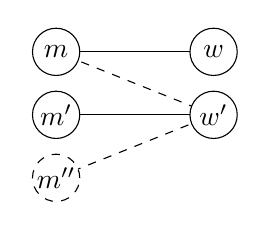
\begin{tikzpicture}
		\draw (0,1.6) node[](m-1){} (2,1.6) node[](w-1){};
		\draw (0,0.8) node[](m-2){} (2,0.8) node[](w-2){};
		\draw (0,0) node[](m-3){};
		\draw (m-1) -- (w-1) (m-2) -- (w-2);
		\draw[dashed] (m-1) -- (w-2) -- (m-3) ;
		\filldraw[fill=white] (m-1) circle (0.3) (m-2) circle (0.3) (w-1) circle (0.3) (w-2) circle (0.3);
		\fill [fill=white] (m-3) circle (0.3);
		\draw [dashed] (m-3) circle (0.3);
		\draw (m-1) node(){$m$} (m-2) node(){$m'$} (w-1) node(){$w$} (w-2) node(){$w'$} (m-3) node(){$m''$};
	\end{tikzpicture}
	\caption{}\label{fig:stable-matching-2}
\end{wrapfigure}
\begin{proof}
	由定理\ref{thm:stable-matching-5},集合$S$是一个完美匹配。所以要证明$S$是一个稳定匹配,我们可以假定$S$中存在不稳定的对,然后推出矛盾。
	假定$S$中有两个匹配对$(m,w)$和$(m',w')$,并且具有下面的特点
	\begin{itemize}[label=$\ast$]
		\item 相比于$w$,$m$更倾向于$w'$
		\item 相比于$m'$,$w'$更倾向于$m$
	\end{itemize}
	在执行算法的过程中,当$m$向$w$提出申请时,$m$是不是已经向$w'$提出过申请?如果没有,那么$w$在$m$的评价中比$w'$更高,这跟我们的假设“相比于$w$,$m$更倾向于$w'$”矛盾。
	如果$m$已经提出过申请,那么他被$w'$选择了更倾向的$m''$时拒绝了。$m'$是$w'$的最终选择,所以$m'$的在$w'$中的排名不会比$m''$低。这与假设“相比于$m'$,$w'$更倾向于$m$”矛盾。
	所以集合$S$中不存在不稳定对,$S$是个稳定匹配。
\end{proof}
下面来说明一下G-S算法得到的解是相同的。书上说有一种简单的方法来证明这一点(\sout{我没看出来})。我们可以证明得到的解具有相同的特征。然后再得到解是相同的。

首先,如果存在一个稳定匹配包含对$(m,w)$,我们可以说$w$是$m$的一个有效同伴。如果$w$是$m$的一个有效同伴,并且在$m$的排名中比$m$的其他的有效同伴都要高,那么可以说$w$是$m$的最佳有效同伴。
我们用$best(m)$来表示$m$的最佳有效同伴。现在假定$S^*$是一个满足$S^*=\{(m,best(m)):m\in M\}$的对集合。我们将要证明下面的定理。
\begin{theorem}{}{stable-matching-7}
	每一次执行G-S算法得到的结果都是集合$S^*$。
\end{theorem}
\begin{wrapfigure}[]{r}{0.25\linewidth}
	\centering
	\begin{tikzpicture}
		%元素关系
		\draw (0,1.6) node[](m-1){} (2,1.6) node[](w-1){};
		\draw (0,0.8) node[](m-2){} (2,0.8) node[](w-2){};
		\draw (0,0) node[](m-3){};
		\draw[dashed] (m-1) -- (w-1) (m-2) -- (w-2);
		\draw (m-2) -- (w-1) ;
		\filldraw[fill=white] (m-1) circle (0.3) (m-2) circle (0.3) (w-1) circle (0.3) (w-2) circle (0.3);
		\fill [fill=white] (m-3) circle (0.3);
		\draw (m-1) node(){$m$} (m-2) node(){$m'$} (w-1) node(){$w$} (w-2) node(){$w'$};
		%图例
		\draw[dashed] (-0.3,0)--(0,0) node[right](){集合$S'$};
		\draw (-0.3,-0.5)--(0,-0.5) node[right](){集合$S$或过程$\varepsilon$};
	\end{tikzpicture}
	\caption{}\label{fig:stable-matching-3}
\end{wrapfigure}
\begin{proof}
	我们假定,某次执行G-S算法得到的匹配$S$,其中存在男性没有匹配到他的最佳有效同伴。我们把这个过程记为$\varepsilon$。既然男性提出申请的次序是沿着倾向列表降序的,
	那也就是说存在男性在$\varepsilon$中被他的有效同伴被拒绝了。%根据定理\ref{thm:stable-matching-2},也就是存在男性$m$被他的最佳有效同伴$ws$拒绝了。
	那么在$\varepsilon$中,记第一个被有效对象拒绝的为$m$,并且被他的有效对象$w$拒绝。
	考虑$m$被$w$拒绝的时刻,要么是因为$w$已经跟排名更高的$m'$成了约定状态,要么是因为排名更高的$m'$向$w$提出了申请。不管怎样,在那个时刻$w$跟$m'$形成或维持约定状态,$m'$在$w$的排名中比$m$要高。

	既然$w$是$m$的一个有效同伴,那么存在一个稳定匹配$S'$包含这个对$(m,w)$。那么,假定这个时候跟$m'$组成对的是$w'$,并且$w‘\neq w$。

	在$\varepsilon$中,$m$是第一个被$w$拒绝的有效对象,那么当$m'$向$w$提出申请的时候还没有被有效对象(比如$w'$)拒绝过,也就是说在$m'$看来$w$的排名比$w'$要高。
	并且$m'$在$w$的排名比$m$要高。那么$(m,w')$在$S'$中倾向成为一对,但$(m,w')\notin S'$,这就是个不稳定因素。

	这跟我们关于$S'$是稳定匹配的声明是矛盾的,因此我们最初的声明是错误的。那么不存在任何过程使得$m$不与最佳有效同伴$best(m)$匹配。
\end{proof}
对于男性,G-S算法得到的是理想的。不幸的是对于女性来说是不一样的。对于一个女性$w$,如果存在一个稳定匹配包含对$(m,w)$,那么我们说$m$是一个有效同伴。如果$m$是$w$的一个有效同伴,
并且对于$w$来说没有有效同伴的排名比$m$低,那我们说$m$是$w$的最差有效同伴。
\begin{theorem}{}{stable-matching-8}
	在稳定匹配$S^*$中,每一个女性都跟她的最差有效同伴匹配。
\end{theorem}
\begin{wrapfigure}[]{r}{0.25\linewidth}
	\centering
	\begin{tikzpicture}
		%元素关系
		\draw (0,1.6) node[](m-1){} (2,1.6) node[](w-1){};
		\draw (0,0.8) node[](m-2){} (2,0.8) node[](w-2){};
		\draw (0,0) node[](m-3){};
		\draw[dashed] (m-1) -- (w-2) (m-2) -- (w-1);
		\draw (m-1) -- (w-1) ;
		\filldraw[fill=white] (m-1) circle (0.3) (m-2) circle (0.3) (w-1) circle (0.3) (w-2) circle (0.3);
		\fill [fill=white] (m-3) circle (0.3);
		\draw (m-1) node(){$m$} (m-2) node(){$m'$} (w-1) node(){$w$} (w-2) node(){$w'$};
		%图例
		\draw[dashed] (-0.3,0)--(0,0) node[right](){集合$S'$};
		\draw (-0.3,-0.5)--(0,-0.5) node[right](){集合$S^*$};
	\end{tikzpicture}
	\caption{}\label{fig:stable-matching-3}
\end{wrapfigure}

\begin{proof}
	假定存在对$(m,w)$在稳定匹配$S^*$中,并且$m$不是$w$的最差有效同伴。那么存在一个稳定匹配$S'$,$w$跟一个比$m$差的人$m'$形成了对。在$S'$中,$m$跟$w'$形成了一对,且$w'\neq w$。
	由定理\ref{thm:stable-matching-7},我们知道$w$是$m$的最佳有效对象,并且$w'$是$m$的有效对象,那么我们可以说相对于$w'$,$m$更倾向于$w$。
	但这会导致$(m,w)$成为$S'$中的不稳定因素,这与$S'$是稳定匹配是矛盾的。因此我们的假设是错误的。即对于在$S^*$中的$(m,w)$,$m$是$w$的最差有效同伴。
\end{proof}

\chapter{图算法之最小生成树}

\begin{introduction}
	\item 问题概述
	\item Prim算法
	\item Kruskal算法
\end{introduction}

\section{概述}
给定一张边带权的无向图G=(V, E),其中V表示图中点的集合,E表示图中边的集合,n=|V|,m=|E|。
由V中的全部n个顶点和E中n-1条边构成的无向连通子图被称为G的一棵生成树,其中边的权值之和最小的生成树被称为无向图G的最小生成树。

最小生成树最为经典的两个算法分别是Prim算法和Kruskal算法。本节将首先讨论这两个算法的执行过程。

\section{基本概念}
在深入探讨之前,还需明白一些定义:

\begin{definition}{path}{path}
	A path is a sequence of edges which connects a sequence of nodes.
\end{definition}

\begin{definition}{cycle}{cycle}
	A cycle is a path with no repeated nodes or edges other than the
starting and ending nodes.
\end{definition}

可以借助\autoref{fig:path-cycle}理解path以及cycle的概念。

\begin{figure}[hbt]
	\centering
	\includegraphics[scale=0.5]{image/pathcycle.png}
	\caption{具体例子说明path和cycle}\label{fig:path-cycle}
\end{figure}

\begin{definition}{cut}{MSTcut}
	A cut is a partition of the nodes into two nonempty subsets S and V / S.
\end{definition}

\begin{definition}{cutset}{MSTcutset}
	The cutset of a cut S is the set of edges with exactly one endpoint in S.
\end{definition}

可以借助\autoref{fig:cut-cutset}理解cut以及cutset的概念。

\begin{figure}[hbt]
	\centering
	\includegraphics[scale=0.5]{image/cutcutset.png}
	\caption{具体例子说明cut与cutset}\label{fig:cut-cutset}
\end{figure}

\begin{theorem}{}{cycle-cutset-theorem}
	A cycle and a cutset intersect in an even number of edges.
\end{theorem}

可以借助\autoref{fig:cycle-cutset}理解\autoref{cycle-cutset-theorem}。

\begin{figure}[hbt]
	\centering
	\includegraphics[scale=0.5]{image/cyclecutset.png}
	\caption{cycle、cutset的性质}\label{fig:cycle-cutset}
\end{figure}

\begin{definition}{生成树}{ST}
Let H = (V, T) be a subgraph of an undirected graph G = (V, E).
H is a spanning tree of G if H is both acyclic and connected.
\end{definition}

一个生成树的例子如\autoref{fig:exampleofST}所示。

\begin{figure}[hbt]
	\centering
	\includegraphics[scale=0.5]{image/exampleofST.png}
	\caption{生成树的例子}\label{fig:exampleofST}
\end{figure}

\begin{theorem}{}{ST-theorem}
	如果H = (V, T)是一个无向图G = (V, E)的子图,那么,以下各条件等价:

	1. H是G的一棵生成树

	2. H是无环且连通的

	3. H是连通的并且有 V – 1条边

	4. H是无环的并且有 V – 1条边

	5. 任意拿掉H的一条边,就不再使其连通

	6. 任意增加一条边,则H就会构成环

\end{theorem}

\begin{definition}{最小生成树}{MST}
	Given a connected, undirected graph G = (V, E) with edge costs $c_e$,
a minimum spanning tree (V, T) is a spanning tree of G such that the sum
of the edge costs in T is minimized.
\end{definition}

一个生成树的例子如\autoref{fig:exampleofMST}所示。

\begin{figure}[hbt]
	\centering
	\includegraphics[scale=0.5]{image/exampleofMST.png}
	\caption{生成树的例子}\label{fig:exampleofMST}
\end{figure}

\begin{theorem}{Cayley’s theorem}{Cayley-theorem}
	The complete graph on n nodes has $n^(n–2)$ spanning trees
\end{theorem}

最小生成树是一个基础却有着十分广泛的应用的问题,之后的\autoref{sec:prim}和\autoref{sec:kruskal}
将分别介绍求解最小生成树的Prim算法和Kruskal算法。

\section{Prim算法}\label{sec:prim}
\subsection{算法描述与演示}
\begin{algorithm}
	\DontPrintSemicolon
	\KwIn{Graph G}
	\KwResult{MST of Graph G}
	\Begin{
		$S \leftarrow \{ s \} $ for any node s,$T \leftarrow \emptyset$;\\
		\For{$|T| < n-1$}{
			Add to T a min-weight edge with exactly one endpoint in S;\\
			Add the other endpoint to S;\\
		}
		Return T ;\\
	}
	\caption{Prim}\label{alg:Prim}
\end{algorithm}

算法执行流程如\autoref{fig:Prim}所示。

\begin{figure}[hbt]
	\centering
	\includegraphics[scale=0.5]{image/prim.png}
	\caption{Prim算法的执行流程}\label{fig:Prim}
\end{figure}

\subsection{算法正确性证明}
\noindent记图G是一个连通图,Y是对p使用prim算法得到的一棵生成树,$Y_1$是p的一棵最小生成树

\noindent1.若Y=$Y_1$,显然prim算法是正确的

\noindent2.若Y≠$Y_1$,可进行如下推导:

a)Y中有$n( n \geq 1 )$条边不存在于$Y_1$中,在构建Y的过程中,第一次遇到这样的一条边时(以e表示),
则e的一个端点u落在V内(V是之前的prim运算得到的一个子顶点集),另一个端点v落在V外

b)$Y_1$是连通的,故$Y_1$中存在u到v的一条的路径,此路径上必然存在一条边f,它的一个端点落在V内,另一个端点落在V外

c)把e加入$Y_1$,去掉f,$Y_1$仍然连通,根据prim算法,权值$W(f) \geq W(e)$,否则e不会被选入V,
如果$W(f)>W(e)$,新构建的树的权值和会比$Y_1$小,而$Y_1$是最小生成树,因此$W(f)>W(e)$不成立,得$W(f)=W(e)$

d)对每一条类似e的边,重复过程c),最终Y和重新构建的的$Y_1$拥有的边完全一致,
新构建的$Y_1$也是最小生成树,因此Y也是最小生成树,证明prim算法正确

\subsection{算法复杂度}
普通堆优化的 Prim 算法复杂度为 $O(mlogn)$,而斐波那契堆优化的 Prim 算法
能达到 $O(m+nlogn)$

\section{Kruskal算法}\label{sec:kruskal}
\subsection{算法描述与演示}
\begin{algorithm}
	\DontPrintSemicolon
	\KwIn{Graph G}
	\KwResult{MST of Graph G}
	\Begin{
		$T \leftarrow \emptyset$;\\
		$S \leftarrow$sort edges by weight;\\
		\While{$e \in S$}{
			\If{$T \cup \{ e \}$ no cycle}{
				$T = T \cup \{ e \};$
			}
			\If{$|T| < n-1$}{
				Return T ;\\
			}
		}
	}
	\caption{kruskal}\label{alg:kruskal}
\end{algorithm}

算法执行流程如\autoref{fig:kruskal}所示。

\begin{figure}[hbt]
	\centering
	\includegraphics[scale=0.5]{image/kruskal.png}
	\caption{Kruskal算法的执行流程}\label{fig:kruskal}
\end{figure}

\subsection{算法正确性证明}
Kruskal算法每次会向T添加一条最小权重的边,并且不能形成环.
对于一棵树而言, 如果有K个节点, 则必然有K-1条边
我们要证明的问题其实是连续添加的边E(l) l=0,1,2...K-1 是一颗最小生成树MST的子集.

对于基本情况, 如果I = 0, 此时为空集,满足条件;

现在我们假设对 $0 \leq m < K-1$, E(m) 已经满足条件,是$T_1$的子集. 我们来看 E(m+1)的情况,
有E(m+1) = E(m) + {e}, e为算法当前新增的最小权重边.此时分两种情况:

1. 如果{e}是$T_1$的子集,那么问题解决;

2. 如果{e}不是$T_1$的子集, 那么我们要证明 E(m+1) 属于一颗其他的MST子集:

因为{e}不是$T_1$的边, 所以 $T_1$ + {e} 必然有环C(性质1), 同时 E(m) 属于 $T_1$ ,
那么在环C上必然有一个{e'} 不属于E(m) (因为如果属于E(m)的化, 那么算法当前选择的{e}会导致一个环, 与性质1违背).

现在我们定义$T_2$ = $T_1$ + {e} - {e'}, 又因为E(m+1) = E(m) + {e} 所以 E(m+1) 属于$T_2$的子集.$T_2$是一颗MST.

因为{e} 和 {e'} 都不属于 E(m), 算法当前选择的是{e} 说明 $weight({e'}) \geq weight({e})$.
所以我们看$weight(T_2) = weight(T_1) + weight({e}) - weight({e'}) \leq weight(T_1)$ .

这意味着$T_1$是$T_2$的权重upper-bound, 但由于$T_1$已经是MST, 所以必然的$T_2$也是MST. 至此得证.

\subsection{算法复杂度分析及优化}
\begin{theorem}{}{Kruskal-theorem}
	Kruskal’s algorithm can be implemented to run in $O(m log m)$ time.
\end{theorem}

1. Sort edges by cost:$O(m log m)$.

2. Use union–find data structure to dynamically maintain connected components:$O(m \alpha (n))$.

注: $\alpha (n)$是反阿克曼函数,阿克曼函数 $A(m,n)$ 增长极快,其反函数几乎是常数。

下面将简要介绍并查集(union–find data structure)有关内容。
\subsection{并查集}
在计算机科学中,并查集是一种树型的数据结构,用于处理一些不交集(Disjoint Sets)的合并及查询问题。
有一个联合-查找算法(union-find algorithm)定义了两个用于此数据结构的操作:

Find:确定元素属于哪一个子集。它可以被用来确定两个元素是否属于同一子集。

Union:将两个子集合并成同一个集合。

在并查集森林中,每个集合的代表即是集合的根节点。“查找”根据其父节点的引用向根行进直到到底树根。
“联合”将两棵树合并到一起,这通过将一棵树的根连接到另一棵树的根。实现这样操作的一种方法是

\begin{lstlisting}
function MakeSet(x)
     x.parent := x

function Find(x)
     if x.parent == x
        return x
     else
        return Find(x.parent)

function Union(x, y)
     xRoot := Find(x)
     yRoot := Find(y)
     xRoot.parent := yRoot
\end{lstlisting}

这是并查集森林的最基础的表示方法,这个方法不会比链表法好,这是因为创建的树可能会严重不平衡;然而,可以用两种办法优化。

第一种方法,称为“按秩合并”,即总是将更小的树连接至更大的树上。因为影响运行时间的是树的深度,
更小的树添加到更深的树的根上将不会增加秩除非它们的秩相同。在这个算法中,术语“秩”替代了“深度”,因为同时应用了路径压缩时秩将不会与高度相同。

第二个优化,称为“路径压缩”,是一种在执行“查找”时扁平化树结构的方法。关键在于在路径上的每个节点都可以直接连接到根上;
他们都有同样的表示方法。为了达到这样的效果,Find递归地经过树,改变每一个节点的引用到根节点。得到的树将更加扁平。

\chapter{最小生成树其他算法}

\begin{introduction}
	\item red/blue算法
	\item Boruvka算法
\end{introduction}

本章将介绍求解最小生成树的red/blue算法和Boruvka算法。

\section{red/blue算法}

\subsection{基本概念}
下面给出red/blue算法有关内容的定义
\begin{definition}{割(cut)}{cut}
	S$\in$V,S$\neq \emptyset$,点集V被划分成互补的子集S和V/S。
\end{definition}

\begin{definition}{割边集(cutset)}{cutset}
    对于图G的顶点集V的割X、Y,图G的边集E中连接两集合X、Y的所有边的集合叫做这个割的割边集(cutset)。
\end{definition}

\begin{definition}{Red Rule}{Red Rule}
    找到图G中不含红色边的环C,从C中未被染色的边中选出边权最大的边将其染成红色。
\end{definition}

\begin{definition}{Blue Rule}{Blue Rule}
    找到图G中不含蓝色边的割边集D,从D中未被染色的边中选出边权最小的边将其染成蓝色。
\end{definition}

\subsection{算法运行步骤}
\begin{enumerate}
	\item 初始化:对于给定的图G,将所有边标记为未染色。
	\item 在图G中同时运行Red Rule和Blue Rule (可并行运行),直到所有边均被染色为止。
	\item 图G中所有的蓝色边即为图G的最小生成树。
\end{enumerate}

算法具体执行过程如\autoref{fig:redblue}
\begin{figure}[hbt]
	\centering
	\includegraphics[scale=0.4]{image/redblue.png}
  \caption{red/blue算法执行过程图解}\label{fig:redblue}
\end{figure}

\subsection{算法正确性证明}\label{sec:redblue-proof}
\begin{enumerate}
	\item 最优性:Blue Rule染色所得边为最小边

对于图G中的一个割边集D及D中边权最小的边minEdge,如果在Blue Rule运行过程中被染色的是割边集D的其他边biggerEdge,
则可以在最后得到的MST中将biggerEdge从中删除然后将minEdge加入到MST中,可以得到更小的最小生成树。产生矛盾。所以Blue Rule染色所得边为最小边。
\item 合法性:算法所得所有蓝边为无环连通图

由于Blue Rule可知每次选边都不会成环。下证所得为连通图,假设最后所得所有蓝边构成的图不连通或仍然有点未被蓝边连接。

对于第一种情况,则任选某一蓝边的一个顶点并从该顶点开始的所有能通过蓝边的顶点记为集合X,
S与V/S构成图G的一个割,由Red Rule中所选环C不含红色边可知其割边集不可能全部被染成红色,则说明一定有未染色的边,再应用一次Blue Rule即可增大S的点的个数,
重复上述过程直到S=E;对于第二种情况,由于孤立点必不可能在某个环中,所以连接该点的边一定不会被Red Rule染成红色,所以此时应用一次Blue Rule即可使得该点被蓝边连接。综上,算法所得所有蓝边为连通图
\end{enumerate}

\section{Boruvka算法}
\subsection{算法运行步骤}
\begin{enumerate}
	\item 初始化:对于给定的图G,将所有边标记为未染色;将每个顶点作为一个连通块。
	\item 对于所有蓝边连成的连通块应用Blue Rule并将所有Blue Rule选中的边染成蓝色,直到只有一个连通块。
	\item 最后得到的蓝边连成的连通块即为图G的最小生成树。
\end{enumerate}

算法具体执行过程如\autoref{fig:boruvka}
\begin{figure}[h]
	\centering
	\includegraphics[scale=0.4]{image/boruvka.png}
  \caption{boruvka算法执行过程图解}\label{fig:boruvka}
\end{figure}

算法复杂度分析:每次应用Blue Rule后连通块数量至少减半,每次都要遍历所有边,所以算法串行时间复杂度为O(E$\log V$),并行时间复杂度为O(E)。

\subsection{算法正确性证明}
\begin{enumerate}
	\item 最优性:根据~\ref{sec:redblue-proof}中的证明:Blue Rule染色所得边为最小边。
	\item 合法性:一定不会构成环。如果存在环说明一个点的最小连边有两个,与Blue Rule矛盾。
\end{enumerate}

\chapter{分治算法之平面最近点对问题}

\begin{introduction}
\item 平面最近点对问题定义
\item 分治算法设计及伪代码
\item 分治算法正确性证明及复杂度分析
\end{introduction}

\section{平面最近点对问题定义}
给定二维平面上的$n(n \ge 2)$个不同的点$p$组成点集$P = \{p_i \big| 1\le i \le n\}$,
设计算法寻找欧式距离最近的点对$(A,B)$。
\begin{figure}[htb]
    \centering
    \includegraphics[scale=0.5]{Ln9.image/NearestPointsDef.png}
    \caption{问题定义图例}\label{fig1}
\end{figure}

如上图\autoref{fig1}中点对$(A,B)$即为问题的答案。

\section{分治算法设计及伪代码}
对于这样一个问题,我们很直接地可以使用BF (Brute Force)算法进行暴力求解,
即二重循环计算所有点之间的距离,从而获得最小距离,显然该算法的时间复杂度为
$O(n^2)$。那么有没有更快的算法呢?本章我们使用经典的算法思想——分治,
设计一个$O(n\log n)$的算法。

\subsection{分治问题}
遵循分治思想,我们首先要考虑如何分治问题使得问题规模约减。

我们使用X坐标作为第一关键字、Y坐标作为第二关键字,对点集$P$进行排序,
并以点$p_{\lfloor\frac{n}{2}\rfloor}$作为分治点,获得如下两个点集:
\begin{equation*}
    P_1 = \{p_i\ \big|\ 1 \le i \le \lfloor\frac{n}{2}\rfloor \}
\end{equation*}
\begin{equation*}
    P_2 = \{p_i\ \big|\ \lfloor\frac{n}{2}\rfloor < i \le n\}
\end{equation*}
这样就将当前问题约减为两个规模为$\lfloor\frac{n}{2}\rfloor$的子问题。
分治过程如\autoref{fig2}中所示。

\begin{figure}[htb]
    \centering
    \includegraphics[scale=0.5]{Ln9.image/NearestPointsDivide.png}
    \caption{分治过程图例}\label{fig2}
\end{figure}

如此递归下去,我们可以求得两个点集相对应的最近点对距离$\delta_1, \delta_2$,取其中较小值
记为$\delta = \min \{ \delta_1 , \delta_2 \}$。


\subsection{合并结果}

接着,我们需要考虑如何合并子问题的解。

上述的$\delta$一定是正确的合并结果嘛?显然不是,我们并没有考虑,一端在$P_1$,
一端在$P_2$的线段。因此,在合并阶段,我们要将这种情况考虑在内。

这里,我们将所有横坐标与分治点$p_{\lfloor\frac{n}{2}\rfloor}$的横坐标
$x_{\lfloor\frac{n}{2}\rfloor}$差值小于$\delta$的点组成集合$B$,即
\begin{equation*}
    B = \{p_i\ \big|\ 
        \left|x_i - x_{\lfloor\frac{n}{2}\rfloor}\right| \le \delta ,\
        1 \le i \le n\}
\end{equation*}   
因为只有$B$集合中的点之间的距离才有可能小于$\delta$。
$B$集合如下图\autoref{fig3}中阴影部分所示:
\begin{figure}[htb]
    \centering
    \includegraphics[scale=0.5]{Ln9.image/NearestPointsMerge.png}
    \caption{合并过程图例}\label{fig3}
\end{figure}

进一步,我们的目标是检验在$B$集合中是否存在距离比$\delta$更近的点对,以此更新当前问题的解
。因此,对于每个$p_i = (x_i, y_i) \in B$遍历所有在其之下竖直距离不超过$\delta$的点,
即遍历集合
\begin{equation*}
    C(p_i) = \{ p_j\ \big|\ y_i - \delta \le y_j \le y_i, p_j \in B \}
\end{equation*}
为了方便遍历,这里需要对$B$集合中的点,以Y坐标为第一关键字,X坐标为第二关键字,进行排序。

至此,我们完成了父问题的分治与子问题的合并。

\subsection{伪代码}
\begin{algorithm}
    \DontPrintSemicolon{}
    \KwData{Point Set $P = \{p_i\ \big|\ 1 \le i\le n, p_i = (x_i, y_i)\}$}
    \KwResult{the nearest pair $(A, B)$}
\Begin{
    Sort points in $P$ by x-coordinate in descending order\;
    $m \leftarrow \lfloor \frac{n}{2} \rfloor$\;
    $\delta_1 \leftarrow \text{Nearest-Pair}(P[1,\ \ldots,\ m])$\;
    $\delta_2 \leftarrow \text{Nearest-Pair}(P[m + 1,\ \ldots ,\ n])$\;
    $\delta \leftarrow \min \{ \delta_1, \delta_2 \}$\;
    $B \leftarrow \{ \}$\;
    \ForEach{$p_i\in P$}{
        \If{$\left| x_i - x_m\right| \le \delta$}{
            $\text{add } p_i \text{ to } B$
        }
    }
    Sort points in $B$ by y-coordinate in descending order\;
    \For{$i \leftarrow 1 $ \KwTo$|B|$}{
        \For{$j \leftarrow i + 1$ \KwTo$|B|$} {
            \If{$\left| y_i - y_j \right| \le \delta$}{
                $\delta \leftarrow \min \{ \delta ,\ \text{Euclidean-Distance}(p_i,\ p_j) \}$
            }
        }
    }
    Return $\delta$
}
\caption{Nearest-Pair\label{NPP}}
\end{algorithm}

\section{分治算法正确性证明与复杂度分析}

\sum_{n = 1}^{\infty}  \chapter{分治法之大数乘法}
\begin{introduction}
	\item 问题背景
	\item 直接分治法
	\item 改进分治法
\end{introduction}

\section{问题描述}
给定两个大数$A$和$B$, 试计算
\begin{math}
	A \times B
\end{math}.
其中$A$和$B$分别表示为
\begin{math}
	A = a_n a_{n-1} a_{n-2} \ldots a_2 a_1
\end{math}
,
\begin{math}
	B = b_n b_{n-1} b_{n-2} \ldots b_2 b_1
\end{math}.
根据已学知识,给出如下引理。

\begin{lemma}{}{label_for_a+b}
	直接计算$A + B$,其复杂度为$O(n)$, 其中$n$为$A$和$B$的十进制位数。
\end{lemma}

直接计算$A \times B$时,我们将$A$与$B$的各位相乘,在将各中间结果相加,得到最终结果。
不难得出,这一过程需要进行$n$次基本乘法与$n+1$次加法。
根据引理\ref{lem:label_for_a+b},有:
\begin{theorem}{}{label_for_a*b}
	直接计算$A \times B$的时间复杂度为$O(n^2)$.
\end{theorem}

由定理\ref{thm:label_for_a*b}和引理\ref{lem:label_for_a+b}可知,如果我们直接相乘两个大数,其时间复杂度相比加法运算高出一个量级。
由于乘法在计算机中大量存在,我们希望找到更好的算法来降低乘法计算的时间复杂度,以提升计算机的性能。
分治法为我们提供了一条途径。
\section{直接分治法}
\subsection{算法描述}
这是一种简单的分治方法,将两个大数分为前后两部分,进行相乘。不失一般性,这里假设$n$为偶数。
将$A$与$B$分割为$A_2$, $A_1$, $B_2$, $B_1$,即:
\begin{displaymath}
	\begin{split}
		A_2 &= a_{n} a_{n-1} \ldots a_{\frac{n}{2} + 2} a_{\frac{n}{2} + 1}\\
		A_1 &= a_{\frac{n}{2}} a_{\frac{n}{2} - 1} \ldots a_2 a_1\\
		B_2 &= b_{n} b_{n-1} \ldots b_{\frac{n}{2} + 2} b_{\frac{n}{2} + 1}\\
		B_1 &= b_{\frac{n}{2}} b_{\frac{n}{2} - 1} \ldots b_2 b_1
	\end{split}
\end{displaymath}

则$A$可以写为$A = A_2 \times 2^{\frac{n}{2}} + A_1$.
$B$可以写为$B = B_2 \times 2^{\frac{n}{2}} + B_1$.
计算$A \times B$的问题在进行上述转换后表示为:
\begin{displaymath}
	\begin{split}
		A \times B
		& = (A_2 \times 2^{\frac{n}{2}} + A_1) \times (B_2 \times 2^{\frac{n}{2}} + B_1) \\
		& = A_2 B_2 \times 2^n + (A_2 B_1 + A_1 B_2) \times 2^{\frac{n}{2}} + A_1 B_1
	\end{split}
\end{displaymath}

此时将两个大数相乘的问题转化为4个乘法子问题和3个加法子问题。显然,分治策略还可以对子问题使用,继续减小问题的规模。

\subsection{伪代码}
\begin{algorithm}
	\DontPrintSemicolon{}
	\KwIn{Two large numbers $A$, $B$, which both have $n$ decimal digits}
	\KwResult{$A \times B$}
	\Begin{
		$n \leftarrow $ Number of Decimal Digits of $A$ and $B$\;
		\If{$n \neq 1$}{
			Divide $A$, $B$ into $A_2$, $A_1$, $B_2$ and $B_1$\;
			$C_3 \leftarrow DirectDAC(A_2, B_2)$\;
			$C_2 \leftarrow DirectDAC(A_2, B_1)$\;
			$C_1 \leftarrow DirectDAC(A_1, B_2)$\;
			$C_0 \leftarrow DirectDAC(A_1, B_1)$\;
			\KwRet{$C_3 \ll n + (C_2 + C_1) \ll (\frac{n}{2}) + C_0$}\;
		}
		\Else{
			\KwRet{$A \times B$}
		}
	}
	\caption{DirectDAC\label{label_for_pseudo_DirectDAC}}
\end{algorithm}

\subsection{复杂度分析}
由上述的算法描述可知,算法的主要开销来自于每次分支带来的4个乘法子问题和3个加法子问题,由于移位可在机器中由一个简单的指令完成,我们忽略这个操作的时间。\\
假设$T(n)$表示两个$n$位大数相乘所需的时间开销,则在直接分治法中:
\begin{displaymath}
	\begin{split}
		T(n)
		&= 4T(\frac{n}{2}) + 3n \\
		&= 4T(\frac{n}{2}) + O(n)
	\end{split}
\end{displaymath}

根据主方法,$\log_2 4  = 2> 1$, 推出如下定理:
\begin{theorem}{}{label_for_DirectDAC_complexity}
	用直接分治法计算$A \times B$的时间复杂度为$O(n^2)$.
\end{theorem}

根据定理\ref{thm:label_for_DirectDAC_complexity},直接分治法的性能是令人失望的,因为其并不能提供时间上优于直接相乘的性能。
但分治策略提示我们,这个算法的性能与乘法子问题的数目强相关。我们如果能够用一些其他的开销换取更少的乘法子问题数目,也许能得到更好的算法。


\newpage
\section{改进分治法}
\subsection{改进思路}
在直接分治法中,通过对大数进行分割,我们有:
\begin{displaymath}
	A \times B = A_2 B_2 \times 2^n + (A_2 B_1 + A_1 B_2) \times 2^{\frac{n}{2}} + A_1 B_1
\end{displaymath}

这个过程中,引入了4次乘法运算;在上一节中提到,分治策略和主定理提示我们尽可能减少乘法的次数。
但换取更低的乘法子问题数,需要其他的开销。
一种想法是,由于加法的复杂度为$O(n)$,我们也许可以用略多的加法子问题,来减少乘法子问题数。
基于此想法,我们对直接分治法作出一些改进。首先将直接分治法中的计算式修改为:
\begin{displaymath}
	\begin{split}
		A \times B
		&= A_2 B_2 \times 2^n + (A_2 B_1 + A_1 B_2) \times 2^{\frac{n}{2}} + A_1 B_1\\
		&= A_2 B_2 \times 2^n + ((A_2 + A_1)\times(B_2 + B_1) - A_2 B_2 - (A_1 B_1)) \times 2^{\frac{n}{2}} + A_1 B_1
	\end{split}
\end{displaymath}

观察上式,我们只需要做3次乘法,即计算$A_2 B_2$, $A_1 B_1$, $(A_2 + A_1)\times(B_2 + B_1)$, 以及4次加法,2次减法。
考虑到加法和减法本质上等同,我们成功地将这一问题转化为了3个乘法子问题和6个加法子问题。相比于直接分治法,我们降低了乘法的数量。

下面给出该算法的伪代码及复杂度分析。
\subsection{伪代码}
\begin{algorithm}
	\DontPrintSemicolon{}
	\KwIn{Two large numbers $A$, $B$, which both have $n$ decimal digits}
	\KwResult{$A \times B$}
	\Begin{
		$n \leftarrow $ Number of Decimal Digits of $A$ and $B$\;
		\If{$n \neq 1$}{
			Divide $A$, $B$ into $A_2$, $A_1$, $B_2$ and $B_1$\;
			$C_2 \leftarrow DirectDAC(A_2, B_2)$\;
			$C_1 \leftarrow DirectDAC(A_1, B_1)$\;
			$C_0 \leftarrow DirectDAC(A_2 + A_1, B_2 + B_1)$\;
			\KwRet{$C_2 \ll n + (C_0 - C_2 - C_1) \ll (\frac{n}{2}) + C_1$}\;
		}
		\Else{
			\KwRet{$A \times B$}
		}
	}
	\caption{ModifiedDAC\label{label_for_pseudo_ModifiedDAC}}
\end{algorithm}

\subsection{复杂度分析}
同上节的复杂度分析,我们此处也忽略移位操作带来的开销。改进分治法中,我们将问题分解为3个乘法子问题与6个加法子问题。
因此有:
\begin{displaymath}
	\begin{split}
		T(n)
		&= 3T(\frac{n}{2}) + 6n\\
		&= 3T(\frac{n}{2}) + O(n)
	\end{split}
\end{displaymath}

根据主方法,$\log_2 3 > 1$. 推出如下定理:
\begin{theorem}{}{label_for_ModifiedDAC_complexity}
	用改进分治法计算$A \times B$的时间复杂度为$O(n^{\log_2 3}) \approx O(n^{1.585})$.
\end{theorem}

\chapter{动态规划(1)}

\begin{introduction}
  \item 带权区间调度
  \item 矩阵链乘法
\end{introduction}

\section{概述}
在前面的课程中,已经学习过了贪心法和分治法两种策略,本章将开始动态规划(Dynamic programming)的学习。
简要比较一下几种算法策略的不同。

\begin{itemize}
  \item 贪心法 -基于贪心策略,每次总是选取眼前最优的选项,同时期待最终的结果最优。
        优点在于思考和模型建立较为简单,难点在于如何证明算法的正确性。
  \item 分治法 -分而治之,子问题不存在重叠。
        难点在于如何分割问题,以及如何合并解。
  \item 动态规划 -思想类似于分治,与贪心法相反,子问题之间存在重叠,算法执行过程中记录子问题的解。
        难点在于如何找到转移方程。
\end{itemize}

本章将介绍动态规划在带权区间调度~\ref{sec:weighted-interval-scheduling} 、矩阵链乘法~\ref{sec:matrix-chain-multiplication} 两个问题上的应用。

\section{带权区间调度}\label{sec:weighted-interval-scheduling}

\subsection{问题描述}

\begin{figure}[hbt!]
  \centering
  \begin{tikzpicture}
    \draw[|-|] (0, 5) -- node [above] {$w_1=2$} (2, 5);
    \draw[|-|] (1, 4) -- node [above] {$w_2=4$} (5, 4);
    \draw[|-|] (3, 3) -- node [above] {$w_3=4$} (7, 3);
    \draw[|-|] (1.5, 2) -- node [above] {$w_4=7$} (8.5, 2);
    \draw[|-|] (8, 1) -- node [above] {$w_5=2$} (10, 1);
    \draw[|-|] (9.5, 0) -- node [above] {$w_6=1$} (10.5, 0);
  \end{tikzpicture}
  \caption{区间调度示例}\label{fig:wis-picture-1}
\end{figure}

下面给出带权区间调度问题的定义。

\begin{definition}{带权区间调度问题}{def:weighted-interval-scheduling}
  给定区间$I_1, I_2, \ldots, I_n$,
  $s_i$为$I_i$开始时间,$f_i$为$I_i$的结束时间($f_i>s_i$),$w_i>0$, 假设$\forall i < j$,$ s_i<s_j$。
  \begin{itemize}
    \item $OPT(k)$:表示区间集合$\{ I_1, I_2, \ldots , I_i \}$上的最优解权值。
    \item $P(i)$:表示$I_i$的前驱,当$P(i)=j$时,有$f_j=\max\limits_{1 \leq k < i}\{f_k | f_k < s_i\}$,当$I_i$没有前驱时,$P(i)=0$
  \end{itemize}
  目标:寻找一个$\sum w_i$最大的区间子集$R$,满足$\forall I_m,I_n \in R, m < n \text{都有} f_m < s_n$。
\end{definition}

通俗来讲,就是找出一个彼此时间不重叠的区间序列,使得这个序列的权重在所有可能的序列中,权重最大。

\begin{remark}
  以\autoref{fig:wis-picture-1}为例,$P(6)=4, P(5)=3, P(4)=0, P(3)=1, P(2)=0, P(1)=0$
\end{remark}

\subsection{贪心}

\begin{figure}[hbt!]
  \centering
  \begin{subfigure}{.3\textwidth}
    \centering
    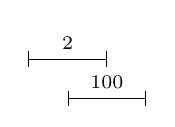
\begin{tikzpicture}
      \draw[|-|] (0, 0) -- node [above] {\scriptsize 2} (1, 0);
      \draw[|-|] (0.5 , -0.5) -- node [above] {\scriptsize 100} (1.5, -0.5);
    \end{tikzpicture}
    \caption{}\label{fig:wis-counterexample1}
  \end{subfigure}
  \begin{subfigure}{.3\textwidth}
    \centering
    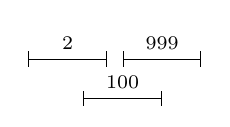
\begin{tikzpicture}
      \draw[|-|] (0, 0) -- node [above] {\scriptsize 2} (1, 0);
      \draw[|-|] (1.2, 0) -- node [above] {\scriptsize 999} (2.2, 0);
      \draw[|-|] (0.7 , -0.5) -- node [above] {\scriptsize 100} (1.7, -0.5);
    \end{tikzpicture}
    \caption{}\label{fig:wis-counterexample2}
  \end{subfigure}
  \begin{subfigure}{.3\textwidth}
    \centering
    \begin{tikzpicture}
      \draw[|-|] (0, 0) -- node [above] {\scriptsize 2} (1, 0);
      \draw[|-|] (1.2, 0) -- node [above] {\scriptsize 3} (2.2, 0);
      \draw[|-|] (0.7 , -0.5) -- node [above] {\scriptsize 6} (1.7, -0.5);
    \end{tikzpicture}
    \caption{}\label{fig:wis-counterexample3}
  \end{subfigure}
  \caption{贪心反例}\label{fig:wis-counterexample}
\end{figure}

\begin{enumerate}
  \item 以最早完成时间排序,反例如\autoref{fig:wis-counterexample1}
  \item 以最大权重排序,反例如\autoref{fig:wis-counterexample2}
  \item 选择冲突最少的区间,反例如\autoref{fig:wis-counterexample3}
\end{enumerate}

常见的贪心思考方向无法解决带权区间调度问题。

\subsection{动态规划}

\subsubsection{算法设计}
观察带权区间调度问题,对于最优解$OPT(n)$,可以得到如下两个结论:
\begin{itemize}
  \item 子集$R$要么包含$I_n$,要么不包含$I_n$
  \item 对于区间$I_n$
        \begin{itemize}
          \item 如果$I_n \in R$,$OPT(n)=w_n+OPT(P(n))$
          \item 如果$I_n \notin R$,$OPT(n)=OPT(n-1)$
        \end{itemize}
\end{itemize}

于是我们可以得到该问题的状态转移方程:
\begin{equation}
  OPT(n) = \begin{cases}
    w_n + OPT(P(n)), & I_n \in R    \\
    OPT(n-1),        & I_n \notin R
  \end{cases}
\end{equation}
\par
因为需要找到最大的权值,上式也可以写成
\begin{equation}
  OPT(n)=\max \{w_n+OPT(P(n)),OPT(n-1)\}
\end{equation}

\subsubsection{算法分析}

\paragraph*{时间复杂度}
在记录最优解的情况下,仅需要填满大小为$n$的一维数组即可,每次计算$OPT(n)$时会从数组中取已计算的$OPT(n-1)$,因此时间复杂度为$O(n)$。
考虑不记录子问题解的情况,在最坏情况下$T(n)=T(n-1)+T(n-2)$,可以发现这是一个斐波那契序列,因此求解该问题的时间复杂度约为$O(1.618^n)$。
\paragraph*{空间复杂度}
算法执行过程中,会开辟一个空间记录子问题最优解,即空间复杂度为$O(n)$。

\section{矩阵链乘法}\label{sec:matrix-chain-multiplication}

\subsection{问题描述}
假设有矩阵乘法$A \cdot B \cdot C$。其中$A = (n \times m), B = (m \times n), C = (n \times m)$。
根据矩阵乘法性质,有$(A \cdot B) \cdot C = A \cdot (B \cdot C)$。
前者的时间复杂度为$O(2n^2m)$,后者的时间复杂度为$O(2m^2n)$。
于是我们可以看出,不同的矩阵相乘顺序,对结果没有影响,但是对计算时间却有较大的影响,矩阵链乘法即是找到一个最优的相乘顺序。
\par
下面给出矩阵链乘法问题的相关定义。
\begin{definition}{矩阵链乘法问题}{def:matrix-chain-multiplication}
  给定n个矩阵的链$<A_1,A_2,\ldots,A_n>$矩阵$A_i$的规模为$p_{i-1} \times p_i, (1 \leq i \leq n)$。
  求完全括号化方案,使得计算矩阵乘积$A_1 \cdot A_2 \cdot A_3 \cdots A_n$所需的标量乘法次数最少。
  \begin{itemize}
    \item $C(i,j,k)$:记$\underbrace{(A_i \cdot A_{i+1} \cdots A_j)}_{p \times q}  \cdot \underbrace{(A_{j+1} \cdot A_{j+2} \cdots A_k)}_{q \times r}$相乘的代价为$C(i,j,k)=pqr$。
    \item $OPT(i,j)$:记矩阵链$<A_i \cdots A_j>$之间的最优相乘成本为$OPT(i,j)$。
  \end{itemize}
\end{definition}

\subsection{算法设计}
对于矩阵链$<A_i \cdots A_j>$,我们可以在$i$到$j$之间找到一个切分点$k$,将问题分解为$<A_i \cdots A_k>$和$<A_{k+1} \cdots A_j>$两个子问题。
假设这两个子问题的最优解已知(在动态规划中,可以理解为已存在子问题解的记录),那么可以得到如下的公式。
\begin{equation}
  OPT(i,j) = \begin{cases}
    0,                                                            & i = j \\
    \min\limits_{i \leq k < j} \{ OPT(i,k)+OPT(k+1,j)+C(i,k,j)\}, & i < j
  \end{cases}
\end{equation}

\begin{remark}
  根据算法执行的迭代方向不同,公式可以有多种写法,几种迭代方向参见\autoref{fig:mcm-fig1}
\end{remark}

\begin{algorithm}
  \caption{MATRIX-CHAIN-ORDER}\label{alg:mco}
  \KwIn{序列$p=<p_0,p_1,\ldots,p_n>$,长度为$n+1$,$p_{i-1} \times p_i$为第$i$个矩阵的规模}
  \KwOut{代价表$OPT[1..n, 1..n]$,分割表$s[1..n-1, 2..n]$记录$OPT(i,j)$的分割点$k$}
  \BlankLine{}
  $n = p.length-1$\;
  $\text{let } OPT[1..n, 1..n] \text{ and } s[1..n-1, 2..n] \text{ be new tables}$\;
  \For{$i = 1$ \KwTo$n$}{$OPT[i,i]=0$\;}
  \For{$l = 2$ \KwTo$n$}{
  \For{$i = 1$ \KwTo$n-l+1$}{
  $j = i+l-1$\;
  $OPT[i,j] = \infty$\;
  \For{$k = i$ \KwTo$j-1$}{
  $q = OPT[i,k]+OPT[k+1,j]+p_{i-1} p_k p_j$\;
  \If{$q < OPT[i,j]$}{
    $OPT[i,j] = q$\;
    $s[i,j] = k$\;
  }
  }
  }
  }
  \Return{OPT and s}
\end{algorithm}

\begin{figure}[hbt!]
  \centering
  \includegraphics[scale=0.6]{image/dynamic-programming-1.png}
  \caption{几种不同的迭代方向}\label{fig:mcm-fig1}
\end{figure}

\subsection{算法分析}
\paragraph*{时间复杂度}
简单分析算法\ref{alg:mco}的嵌套循环结构,可以得到算法的运行时间为$O(n^3)$。
循环嵌套的深度为三层,每层的循环变量$(i\text{、}j\text{和}k)$最多取$n-1$个值。
\paragraph*{空间复杂度}
需要$O(n^2)$的空间来保存$OPT$和$s$。
\chapter{字符串编辑距离}

\begin{introduction}
	\item 问题引入
	\item 相关概念
	\item 算法思想
\end{introduction}

\section{问题引入}
如何定义两个字符串的距离呢?ocurrance和occrrence有多大的区别呢?下面我们将讨论两个字符串的距离问题。
\section{相关概念}
\begin{definition}{匹配M}{matching}
	字符串X有$x_1$到$x_n$共n个字符,字符串Y有$y_1$到$y_m$共m个字符。X和Y之间存在一个匹配M,其满足:if(i,j)\in M, (l,k)\in M, $i<l iff j<k$。
\end{definition}

%距离代价:

%$\alpha_{xy}$ :两个不同的字符x和y相匹配的代价,则$\alpha_{xy}=0$.

%$\delta$ :每存在一个没有被选择的字符就会多一个$\delta$.

%总距离代价:所有$\delta$ 和 $\alpha$ 的和。

\begin{definition}{距离代价}{penalty}
$\alpha_{xy}$ :两个不同的字符x和y相匹配的代价,则$\alpha_{xy}=0$.

$\delta$ :每存在一个没有被选择的字符就会多一个$\delta$.

总距离代价:所有$\delta$ 和 $\alpha$ 的和。
\end{definition}

示例:

\begin{figure}[htb]
	\centering
	\includegraphics[scale=0.6]{image/connect1.png}
	\caption{字符串匹配}\label{fig:connect1}
\end{figure}
如上图所示,其中的总距离代价为$\alpha_{ae} + \delta$

\section{算法思想}
从后往前推:

bopt(i,j):字符串$x_1,...,x_i$和$y_1,...,y_j$之间的最佳匹配

 bopt(m,n)=\begin{cases}
 \bopt(m-1,n-1)+\alpha_{x_m y_n}& \text{$x_m$和$y_n$ 相连}\\
 bopt(m-1,n)+\delta& \text{$x_m$跳过}\\
 bopt(m,n-1)+\delta& \text{$y_n$}跳过}
 \end{cases}
 
 从前往后推:
 
 fopt(i,j):字符串$x_i,...,x_m$
 和
 $y_j,...,y_n$
 之间的最佳匹配
 
 fopt(1,1)=\begin{cases}
 \fopt(2,2)+\alpha_{x_1 y_1}& \text{$x_1$和$y_1$ 相连}\\
 fopt(2,1)+\delta& \text{$x_1$跳过}\\
 fopt(1,2)+\delta& \text{$y_1$跳过}
 \end{cases}
 
 初始化:
 bopt(i,0) = \delta_i  $    $bopt(0,i) = \delta_j
 
 构造图:
 
 \begin{figure}[htb]
	\centering
	\includegraphics[scale=0.6]{image/connect2.png}
	\caption{构造图}\label{fig:connect2}
\end{figure}
 按图构造方法如图所示

\chapter{动态规划之最短路径算法}

\begin{introduction}
	\item Dijkstra算法
	\item Bellman-Ford算法
	%\item 提要3
	%\item 提要4
	%\item 提要5
\end{introduction}


\section{最短路径定义}
给的一个带权重的有向图$G=(V,E)$和权重函数$\omega : E\rightarrow R$,该权重函数将每条边映射到实数值的权重上。图中一条路径$p=<v_0,v_1,...,v_k>$的权重$\omega (p)$是构成该路径的所有边的权重之和:$$\omega (p)=\sum\limit_{i=1}^k\omega (v_{i-1},v_i)$$

定义从结点$u$到结点$v$的最短路径权重


\begin{equation}
\delta(u,v) = \begin{cases}
min( \omega (p) : u\stackrel{p}{\longrightarrow} v )  & uv\text{连通} \notag\\
+\infty   &  uv\text{不连通}

\end{cases}
\end{equation}


从结点$u$到结点$v$的最短路径则定义为任何一条权重为$\omega (p)=\delta(u,v)$的从结点$u$到结点$v$的路径$p$

对于每个节点,我们定义两个属性。v.d用来记录源节点s到节点v的最短路径权重上界。v.f用来记录节点v的前驱节点。

定义初始化和松弛两个操作。

\begin{lstlisting}[caption=初始化和松弛伪代码]
INITIALIZE-SINGLE-SOURCE(G,s)
for each vertex v in G.V
         v.d=$\infty$
    v.f=NULL
s.d=0

RELAX(u,v)
if v.d>u.d+(u,v)
       v.d=u.d+(u,v)
	   v.f=u
\end{lstlisting}

\section{Dijkstra算法}
Dijkstra算法解决的是一般情况下的单源最短路径问题,边的权重要求为非负值。

Dijkstra算法在运行过程中关键是维护一个结点的集合$S$。从源节点$s$到该集合中的每个结点之间的最短路径已经找到。该算法重复
从结点集$V-S$中选择离源节点最近的结点$u$加入到集合$S$中。然后重新计算源节点到其余各点的距离。如此以往,直到所有点都加入到集合$S$中。

\begin{lstlisting}[caption=Dijkstra算法伪代码]
DIJKSTRA(G,S)
INITIALIZE-SINGLE-SOURCE(G,s)
S=NULL
Q=G.V
while Q!=NULL
        u=EXTRACT-MIN(Q)
		S=S+u
		for each vertex v in G.Adj[u]
		         RELAX(u,v)

\end{lstlisting}

算法运行过程如下:

\begin{figure}
\centering
\includegraphics[width=10cm,height=5cm]{image/dijkstra1.png}
\caption{一个带权有向图}
\end{figure}
\begin{figure}
\centering
\includegraphics[width=10cm,height=5cm]{image/dijkstra2.png}
\caption{对应Dijkstar算法执行过程表格}
\end{figure}

表的左侧是当前的集合。表中每一行的数字为源点通过集合中的点到各点的当前最短路径距离。在表中加粗的数字对应的节点为该轮中将被加入到集合$S$中节点。

\subsection{时间复杂度}
算法第1行初始化操作所需时间为$\Theta(V)$,第4行循环一共执|V|次,其中第5行操作所需时间为$O(V)$,第7行的for循环在整个算法执行期间一共执行|E|次,故Dijkstra算法的总运行时间为$O(V^2+E)=O(V^2)$

\subsection{正确性证明}
Dijkstra算法使用贪心的策略,每次选择”最近“的节点加入到集合中。下面通过对已经访问的节点数学归纳法证明其正确性。

1. 当只有两个节点的时候,显然成立。

2. 假设n-1个结点时。现在我们选择一条边(v,u),其中节点u是未访问结点中具有最小的u.d的节点,并且$u.d=v.d+\omega(v,u)$。u.d必定是源点到所有未访问中最短路径长度。因为假如有一条更短的路径,假设k是该路径上第一个未访问的节点,这与假设$k.d>u.d$矛盾,所以u.d必定是源点到所有未访问节点中最短路径长度。类似,如果在没有使用未访问节点情况下存在一条到节点u的更短路径,并且如果该路径上最后一个节点是k,则我们有$u.d=k.d+\omega(k,u)$,与前提矛盾。其余未访问节点同理。

综上所述,Dijkstra算法正确。

\section{Bellman-Ford算法}
Bellman-Ford算法解决的是一般情况下的单源最短路径问题,边的权重可以为负值。

由分析可知,s到t的最短路一定是一个简单路径。并且最短路径的边数小于等于n-1(n为节点数)。我们记opt(v,k)为从v到t,边数小于等于k的最短路径。考虑两种情况,一种是最短路径边数小于等于k-1,一种是边数等于k的。
则有
$$opt(v,k)=min(opt(v,k-1),\min \limits_{(v,w)\in E}(opt(w,k-1)+c(v,w)))$$
其中w是与v直接相连的点。

同理还可以记opt(t,k)为从v到t,边数小于等于k的最短路径。则有
$$opt(t,k)=min(opt(t,k-1),\min \limits_{(w,t)\in E}(opt(w,k-1)+c(w,t)))$$

\begin{lstlisting}[caption=Bellman-Ford算法算法伪代码]
BELLMAN-FORD(G,s)

INITIALIZE-SINGLE-SOURCE(G,s)
for i=1 to |G.V|-1
        for each edge(u,v) in G.E
		         RELAX(u,v)
for each edge(u,v) in G.E
         if v.d>u.d+(u,v)
		       return FALSE
return TRUE

\end{lstlisting}

\subsection{时间复杂度}
算法第1行初始化操作所需时间为$\Theta (V)$,第2到4行循环的运行时间为$\Theta (E)$,且一共要进行|V|-1次循环,第5到7行的for循环所需时间为O(E),Bellman-Ford算法的总运行时间为O(VE)。

\subsection{正确性证明}
若某节点和源点不连通,初始化时,除了源点的距离为0外,其他节点的初始化为无穷大。如果不连通,则该节点所在的连通图的任一条边都不会导致更新。

若节点x点与源点连通。每个点都存在自己的最短路,为$(e_0,e_1,e_2,...,e_k)$。显然,源点只要经过|V|-1条边就可到达任一点。

现只需证明,对节点v,每次松弛操作,至少有一条最短边$e_i$的距离被找到,除非已经到达v点。

对于第一次松弛,必定更新和源点s相连的所有出边。由于源点s初始距离是0,和其相连的节点初始距离都是无穷大。而这些相连的出边中,必有一条是节点v的最短路上起始的一条边。则设有节点k,这个节点是节点v最短路上的一共点,由于下一次松弛将更新与k相连的所有点,必能找到下一个点,且也是节点v的最短路径上的一个点。则通过多次松弛可以找出最短路。

综上所述,Bellman-Ford算法正确。

\input{src/LN18-DP-ZeroOneKnapsack.tex}
\chapter{动态规划之上下文无关文法}\label{header-n1150}

\begin{introduction}
	\item 综述
	\item 上下文无关文法及其派生树
	\item CYK算法
\end{introduction}

\section{综述}\label{header-n1151}

\begin{itemize}
\item
  上下文无关语言是一种形式语言(形式语言指在某个字母表上一些有限长字串的集合)。生成这种语言的文法叫做上下文无关文法,常用于计算机中语法分析器(Parsers)的构造。
\item
  关于这个文法的具体使用在编译原理(以及计算理论)课程中会有详细的介绍,在这里我们只简要介绍其基本概念,着重介绍一个和上下文无关文法有关的动态规划算法------CYK算法(The
  CYK Parsing Algorithm)
\end{itemize}

\section{上下文无关文法及其派生树}\label{header-n1157}

\subsection{上下文无关文法}\label{header-n1158}

\begin{itemize}
\item
  下面先举一个上下文无关文法的例子(S为文法的source):
\end{itemize}

\(S\rightarrow aBb\) \quad
\(B\rightarrow aBb|\epsilon\)

\begin{itemize}
\item
  根据这个文法,如果我们想生成串aaabbb,可以进行如下推导:
\end{itemize}

\(S\Rightarrow aBb \Rightarrow aaBbb \Rightarrow aaaBbbb \Rightarrow aaa\epsilon bbb \Rightarrow aaabbb\)

\begin{itemize}
\item
  形式化地,我们将上下文无关文法定义成如下四元组形式:

  \begin{itemize}
  \item
    \(G=(V,T,S,P)\),其中\(G\)代表文法,\(V\)代表文法中的变量,\(T\)代表文法最终到达的常量,\(S\)代表文法的起始变量(source),\(P\)代表由变量和常量生成的文法。
  \item
    具体的,在上述文法中:

    \begin{itemize}
    \item
      \(V=\{S,B\}\)
    \item
      \(T=\{a,b\}\)
    \item
      \(S=\{S\}\)
    \item
      \(P=\{S\rightarrow aBb , B\rightarrow aBb|\epsilon\}\)
    \end{itemize}
  \end{itemize}
\item
  上述上下文无关文法对应语言:\(L=\{a^nb^n|n为大于或等于1的整数\}\)
\end{itemize}

\subsection{派生树}\label{header-n1186}

\begin{itemize}
\item
  上下文无关文法的派生数指的是把由上下文无关文法生成上下文无关语言的过程用树的形式表示出来,比如19.1.1中的文法可以表示成以下派生树:
\end{itemize}

\begin{itemize}
\item
  可以总结出,派生树的画法是,以S(soruce)节点作为根节点,父节点对应文法的左边,子节点对应文法的右边,建立派生树得到最后的串。最后,从左到右叶子结点的值就是最后生成的串。
\end{itemize}

\section{CYK算法}\label{header-n1194}

\begin{itemize}
\item
  CYK算法是一种基于动态规划思想的算法,要解决的问题是:给定串w,测试这个串是否能够用起始变量S生成。其算法的复杂度为\(O(n^3)\)
\item
  CYK算法是由发现相同思想的三个人J. Cocke、 D. Younger和T.
  Kasami的名字来命名的。
\item
  CYK算法不适用于在所有的context free
  language上直接使用,先要转换成乔姆斯基范式(Chomsky Normal
  Form)才能实现。
\end{itemize}

\subsection{CNF(乔姆斯基范式)}\label{header-n1201}

\begin{itemize}
\item
  文法只包含以下两种形式:
\end{itemize}

\(A\rightarrow BC\) \quad
\(A\rightarrow a\)

\begin{itemize}
\item
  概括来说,即只能由变量生成两个变量或者生成一个最终常量
\item
  转换方法如下:

  \begin{itemize}
  \item
    将常量全部添加\(T_a\rightarrow a\)形式,替换其他生成式中所有的常量为变量
  \item
    将文法右侧所有的多变量变成二变量,即把\(A\rightarrow A_0A_1A_2\)替换成\(A\rightarrow A_0B,B\rightarrow A_1A_2\)形式(多变量同理)
  \end{itemize}
\item
  一个转换的例子如下:

  \begin{itemize}
  \item
    原文法:\(S\rightarrow ABa,A\rightarrow aab,B\rightarrow Ac\)
  \item
    转换后文法:\(S\rightarrow AV_1,V_1\rightarrow BT_a,A\rightarrow T_aV_2,V_2\rightarrow T_aT_b,B\rightarrow AT_c,T_a\rightarrow a,T_b\rightarrow b,T_c\rightarrow c\)
  \end{itemize}
\end{itemize}

\subsection{CYK算法的基本内容}\label{header-n1224}

\begin{itemize}
\item
  问题的形式化定义:对于一个上下文无关文法G和一个给定的串\(w=a_1a_2...a_n\),求解是否存在一种推导(或一棵对应的派生树),使得G能够从S(source)生成对应的字串。
\item
  动态规划的做法是,构造一个动态规划的表(这里以n=5为例子),如下图所示。

  \begin{itemize}
  \item
    水平轴对应串\(w=a_1a_2...a_5\)
  \item
    表中\(x_{ij}\)对应着能够满足生成\(A\Rightarrow a_ia_{i+1}...a_j\)的变元A的集合。
  \item
    最后,如果source点S属于集合\(x_{1n}\),证明这个串可以由S生成,否则则不行。
  \end{itemize}
\end{itemize}

\subsection{算法一个具体例子上的执行过程}\label{header-n1238}

\begin{itemize}
\item
  这一小节我们将用一个例子模拟CYK算法的执行过程,下一节将在此基础上归纳写出CYK算法的关键,也就是动态规划算法的转移方程
\item
  考虑以下这个上下文无关文法,我们用其派生树生成了一个长度为7的串,如下图:
\end{itemize}

\begin{itemize}
\item
  对于串\(aaaabab\),我们构造上述所说的动态规划表如下:
\end{itemize}

\begin{itemize}
\item
  对于上述动态规划表给出说明:

  \begin{itemize}
  \item
    首先求解第一行(\(x_{ii}\))有,其对应的集合就是生成字符串中每一个字符(常量)的源头的集合。例如常量a可以由变量A和C生成,所以其集合就是\{A\textbar C\},常量b可以由变量B生成,所以其对应的集合就是\{B\}。
  \item
    从第二行开始,其结果完全依赖于第一行,例如\(x_{12}\)对应着字符串aa,我们将串aa分成两份,有且只能被分割为第一个a和第二个a这一种情况,那么要求解\(x_{12}\)的值,需要做下面两步:

    \begin{itemize}
    \item
      求出\(x_{11}\)和\(x_{22}\)的笛卡尔积。算出结果为\{AA\textbar AC\textbar CA\textbar CC\}。
    \item
      寻找该笛卡尔积中的每一个元素对应的源头。例如AA、AC、CA都没有对应的,则都为空集,AC对应的源头为\{B\}。最后的结果将这四个集合求并集,得到\(x_{12}\)的值为\{B\}
    \end{itemize}
  \item
    第二行其余项的算法同计算\(x_{12}\)类似。
  \item
    第三行开始,每一个串都有多个划分,比如求解\(x_{13}\),对应的串为aaa,我们就有两种划分,aa和a、a和aa,那么求解\(x_{13}\)只用遵循以下步骤即可:

    \begin{itemize}
    \item
      分别用第二行的策略求出\(x_{12}\)和\(x_{33}\)的笛卡尔积,再寻找其源头,得到第一个集合;求出\(x_{11}\)和\(x_{33}\)的笛卡尔积再寻找其源头,得到第二个集合。
    \item
      将上述两个集合求并集得到\(x_{13}\)的结果
    \end{itemize}
  \item
    第三行其余项的算法同理。
  \item
    从第四行开始往上走,处理策略与第三行类似,只不过是对于要求解串的划分情况更多了而已。例如\(x_{15}\)对应aaaab,这个串有4种划分情况,将每种情况的笛卡尔积求源头,得到四个集合,对这四个集合求并集即得到\(x_{15}\)的结果。
  \end{itemize}
\item
  下面我们将给出求解\(x_{ij}\)一般化的公式
\end{itemize}

\subsection{19.3.4 状态转移方程以及算法伪代码}\label{header-n1277}

\begin{itemize}
\item
  由上述举例我们已经了解到了具体的求解\(x_{ij}\)(从生成串的索引i到索引j对应的源头)的方法,这里归纳给出一般化公式即可:

  \begin{itemize}
  \item
    首先给出一个函数souce(s),其中s为一个集合或者一个字符(i=1时候),函数功能是求出s对应的源头的集合,例如\(source(a)=\{A|C\}\),\(source(\{AA|AC|CA|CC\})={B}\)。
  \item
    基于求源头函数给出状态转移方程(假设原始串被存在数组a{[}N{]}中,串长为n,下标从1开始):
  \end{itemize}

  \(x_{ij}=\begin{cases}\bigcup_{k=i}^{k=j}source(x_{ik}\times x_{kj})& \text{j>i}\\source(a[i])& \text{j=i}\end{cases}\)

  \begin{itemize}
  \item
    注:上述公式中\(\times\)符号代表笛卡尔积
  \end{itemize}
\item
  给出算法的为代码如下(假设原始串被存在数组a{[}N{]}中,串长为n,下标从1开始):
\end{itemize}

\begin{lstlisting}[language = C++, caption = 算法伪代码]
context_free(a[N])
{
    int dp[N][N] //存表
    from len=1 to n //按照串长从1到n,横向计算每一行
        from i=1 to n-len+1 //计算每一行,索引值从1开始到n-len+1
            j=i+len-1
            dp[i][j]=compute xij //按照状态转移方程计算dp[i][j]
    if(S belongs to dp[1][n]) //如果起始点S在dp[1][n]中,这个串就可生成,否则不能生成
        return true
    else 
        return false
}
\end{lstlisting}

\subsection{算法复杂度分析}\label{header-n1293}

\begin{itemize}
\item
  算法复杂度分析如下:

  \begin{enumerate}
  \def\labelenumi{\arabic{enumi}.}
  \item
    要构建整张动态规划表,需要循环次数\(O(n^2)\)
  \item
    每一次循环中,执行\(compute\)
    \(x_{ij}\),其中我们语法中变量个数为常数个,即\(O(1)\),其笛卡尔积的复杂度为\(O(1)\times O(1)=O(1)\)。而我们要对每一个笛卡尔积作不相容的合并操作(即合并集合中没有相同元素),最多合并n-1次,每个集合中元素数量为常数级,这一步不相容union复杂度为\(O(n)\)
  \item
    综上,总复杂度为\(O(n)\times O(n^2)=O(n^3)\)
  \end{enumerate}
\end{itemize}

\chapter{网络流应用}

\begin{introduction}
\item 最大二分匹配问题
\item Tiling Problem
\item 棒球比赛
\item 项目选择
\end{introduction}

本章是在基于网络流FF算法的基础上,学习网络流的应用。

\section{最大二分匹配问题}

\begin{definition}{二分图}{label-for-this-def}
    对于无向图G = (V,E),若顶点集V可以分割为两个互不相交子集(X,Y),使得边集E中任意一条边e = (u,v),都可以满足u属于X ,v 属于Y,则称图G为二分图。
\end{definition}

问题:对于给定的G = (V,E),V为Vl并Vr,Vl交Vr为空集,找到Vl到Vr的最大匹配。

\begin{definition}{匹配}{label-for-this-def}
    一边集M为边集E的子集,且M中任意两条边无公用顶点(不相交),则称M为图G的一个匹配。
\end{definition}

\begin{definition}{极大匹配}{label-for-this-def}
    不是其他任何匹配的子集的匹配。
\end{definition}

\begin{definition}{最大匹配}{label-for-this-def}
    极大匹配中包含最多边数的一个匹配称为最大匹配。
\end{definition}

如下图所示,二者都为极大匹配,但是只有左图为最大匹配。

\centerline{\includegraphics[scale=0.4]{Ln11.image/networkflow1.png}}


使用如下图的方法构建网络流,之后使用FF算法求解。

\centerline{\includegraphics[scale=0.4]{Ln11.image/networkflow2.png}}

网络流解决最大二分匹配问题的时间复杂度为:O(mn)。

\begin{lemma}{最大流最小割定理}{label-for-this-def}
    指在一个网络流中,能够从源点到达汇点的最大流量等于如果从网络中移除就能够导致网络流中断的边的集合(对割的另一种理解)的最小容量和。即在任何网络中,最大流的值等于最小割的容量。
\end{lemma}

使用下面一个例子说明该算法的正确性:

\centerline{\includegraphics[scale=0.6]{Ln11.image/networkflow3.png}}
\begin{example}
  如图所示,给定二分图中,点被分为了Vl和Vr两个部分,构造网络流算法,设置一个起点S,且令S到所有的Vl中的点均有路径,容量为1;设置一个终点T,且从Vr中的点到T均有路径,容量为1。同时,所有Vl与Vr之间的路径容量均设为无穷大,由此可以找到该网络流的最大流和最小割。
\end{example}
\begin{itemize}
  \item 因为最大流等价于最小割,对于残差图Gf,从S点可以到达的点构成集合A,其他点构成集合B。
  \item 因为该图为二分图,所以不存在从Al到Bl的路径,同样的,也不存在从Ar到Br的路径。
  \item 因为找到了最小割,而且最小割是有限数,因此不存在从Al到Br的路径(已知Al到Br的边的容量为正无穷)。
  \item 最小割值 C(A,B) = |Bl|(实际为S流入Bl) + |Ar|(实际为Ar流入T) = 最大流 = 最大匹配。
\end{itemize}
对于二分图来说 |最大匹配|=|最小顶点覆盖|。

\begin{definition}{完美匹配}{label-for-this-def}
    所有的点均被匹配,不存在未被匹配的点。
\end{definition}

\begin{definition}{T(A)}{label-for-this-def}
    \(A \subseteq Vl,T(A) = \{b \in Vr | (a,b) \in E \}\)。
\end{definition}

对于一个二分图来说,如果|Vl|=|Vr|=n,并且存在完美匹配,那么任取集合\(A \subseteq Vl,|T(A)| \ge |A|\)。

\begin{theorem}{霍尔定理}{label-for-this-theorem}
    任取\(A\subseteq Vl,若|T(A)| \geq |A|\),则存在完美匹配。
\end{theorem}
证明霍尔定理的正确性(证明其逆否命题正确):
\begin{itemize}
  \item 逆否命题:若不存在完美匹配,则存在集合A,|T(A)| < |A|。
  \item |Vl| = |Vr| = n,所以最大匹配k<n。
  \item 找到A,B(即S-T割),C(A,B) = f(A,B) = k<n。
  \item |Al|+|Bl| = n,|Bl|+|Ar| = k < n。由此可以推出|Al| > |Ar|,可以推出|T(Al)| < |A|。
  \item 因此,逆否命题成立,霍尔定理得证。
\end{itemize}

\section{骨牌问题}
回顾本课程开头提到的骨牌问题,我们试着用网络流的方法再次解决。

\begin{itemize}
  \item 问题描述:在m*n的残缺棋盘(有方格缺失)上,填入1*2大小的矩形骨牌,能否用骨牌将棋盘填满?

  \item 问题建模:沿用之前的处理方法,黑白相间地将棋盘做上标记,这样棋盘的方格会被分为两个集合(B,W)。若|B|不等于|W|,我们可以得出否定的结论;若|B|=|W|=n,则在B和W集之间,相邻的方格连上边,容量正无穷,这样一来,(B,W) 相当于二分匹配中的(Vl,Vr),就相当于解决一个最大二分匹配问题,建模如图。

\end{itemize}
\centerline{\includegraphics[scale=0.6]{Ln11.image/networkflow4.png}}

求得最大流f=n,则表示该棋盘可以用骨牌填满。

算法复杂度分析:F-F算法复杂度为O(mC),在这个模型中,m=n,C<=4n,所以用网络流解决棋盘问题的算法时间复杂度为\(O(n^2)\)。

\section{棒球比赛}
问题描述:有四个棒球队比赛,目前赛场上的得分情况及剩余的场次如下图,问B队有没有机会赢得比赛(并列第一也算赢)?

\centerline{\includegraphics[scale=0.6]{Ln11.image/networkflow5.png}}

问题建模:先计算若B队赢得了剩下所有可赢得的分后的总得分S。称参赛双方相同的比赛为一类比赛。将每类比赛作为顶点,通过容量为该类比赛剩余场数的入边交于源点s,出边指向参赛队伍,容量为正无穷;参赛队伍出边指向汇点t,容量为S-(该队伍的当前得分)。如下图所示。

\centerline{\includegraphics[scale=0.6]{Ln11.image/networkflow6.png}}

求得最大流f = Cin(t) ,Cin(t)即t的流入边容量之和,则表示B有机会赢。

用F-F算法求模型的最大流和最小割,残差图如图

\centerline{\includegraphics[scale=0.6]{Ln11.image/networkflow7.png}}

如果初始状态,B的得分为90,那么B能否获胜?(B有机会获胜)

\section{项目选择问题}
问题描述:有一项目的集合\{1,2,……,n\},项目之间有一定相互制约关系,完成每个项目都有一个价值vi,vi可正可负。现要求一子集A,使得总价值p最大,且A中任一项目的前驱任务(完成一项目之前所必须完成的项目)也必须在A中。

为更好地理解问题,给出一更加具体地例子,下图所示。

\centerline{\includegraphics[scale=0.6]{Ln11.image/networkflow8.png}}

问题建模:由于有先后的制约关系,所以原图应为一个有向图,在此基础上,引入源点s,指向所有价值为负的项目,容量为该项目价值的绝对值;所有价值为正的项目指向汇点t,容量为该项目的价值。对一实例的建模如图。

\centerline{\includegraphics[scale=0.6]{Ln11.image/networkflow9.png}}


用F-F算法求模型的最大流和最小割,残差图下图所示。其中最小割中的集合B所包含的项目即为问题的解。

\centerline{\includegraphics[scale=0.6]{Ln11.image/networkflow10.png}}

结果正确性分析:

解法可行性。该模型s的所有出边容量为有限值,最坏的情况就是所有负价值点都被选入,此时最小割为s所有出边,因此最小割是包含不到无穷大的边的,此解法也就是可行的。

解为最优解。如下图为此模型获得的一般割情形。

\centerline{\includegraphics[scale=0.6]{Ln11.image/networkflow11.png}}

从上图可求此结果的价值:

\begin{equation}
v = (p_{B+}) - (p_{B-}) = (p_+) - (p_{A+}) - (p_{B-}) = (p_+) - [(p_{A+}) + (p_{B-})] = (p_+) - cut
\end{equation}
所以所得价值为一常数减去割,要求maxv,则割要为mincut,即\(maxv = (p_+) -mincut\)


\chapter{网络流应用之图像分割}


\centering 本章简单介绍网络流在图像分割上的应用。


\begin{definition}{背景知识}{def1}
    图像是可以看作由一个个像素组成的巨大图, 将像素一一用边连接起来, 则这些像素点会成为这个巨大图网络的顶点.
    一个图由前景和背景组成, 假设顶点上的值用 $a_i$ 表示, $ 0 \leq a_i \leq 1 $,  $a_i$ 趋近于 0 表示 $a_i$ 为图的背景, $a_i$ 趋近于 1 表示 $a_i$ 为图的前景, 并且设所有属于前景的顶点 $a_i$ 构成集合 A, 所有属于背景的顶点 $a_j$ 构成集合 B.
    假设边上的值用 $w_{ij}$ 表示, $w_{ij}$ 设为边的惩罚值, $w_{ij}$ 趋向于 0 表示“分离” (即 $w_{ij}$ 连接的两个点分别属于前景和背景), $w_{ij}$ 趋向于 1 表示“在一起” (即 $w_{ij}$ 连接的两个点都属于前景或者背景)
    设总的惩罚值为 $ A = \min\left(\sum_{i \epsilon B}a_i +  \sum_{i \epsilon A}(1 - a_j) + \sum_{i \epsilon A, j \epsilon B}w_{ij} \right) $
\end{definition}


\section{问题实例}
\subsection{问题描述}
\begin{itemize}
    \item 对于下面这个图,利用网络流求解该图前景和背景的最大可能
\end{itemize}

\begin{figure}[htb]
	\centering
	\includegraphics[scale=0.6]{image/Image-segmentation2.png}
	\caption{图片前景背景识别}\label{fig1}
\end{figure}

\subsection{思路描述}
\begin{itemize}
    \item 图形切割算法通过向图 G (V,E) 添加 S 点和 T 点,将图中所有的顶点,与 S 和 T 建立边,
          如果一个点与 S 相连,则对应边的权值为该点的值 $a_i$, 如果一个点与 T 相连,则对应边的权值为1减去该点的值 $ 1 - a_j $。
          可以得到下面这个图:
\end{itemize}

\begin{figure}[htb]
    \centering
    \includegraphics[height=4.5cm]{image/Image-segmentation3.png}
    \caption{图片前景背景识别}\label{fig2}
\end{figure}

\begin{itemize}
    \item   根据最大流最小割, 可以得到得到二分图的最大匹配, 可以得到集合A和B, 保证总的惩罚值 $ A = \min\left(\sum_{i \epsilon B}a_i +  \sum_{i \epsilon A}(1 - a_j) + \sum_{i \epsilon A, j \epsilon B}w_{ij} \right) $ 最小, 
            最小为 $(0.2 + 0.1) + (1 - 0.9) + (1 - 0.8) + 0.3 + 0.3 = 1.2 $, 而 A 和 B 分别对应图的前景和背景。
\end{itemize}



\section{问题扩展}
\begin{itemize}
    \item 假如一个图的前景不是一个整体,
          而是有两个分开的部分,比如两只在两个不同位置的猫在一个图中。
          这样一个算法能否将图像上的前景和背景分开?
\end{itemize}

\begin{figure}[htb]
	\centering
	\includegraphics[scale=0.6]{image/Image-segmentation1.png}
	\caption{图片前景背景识别}\label{fig3}
\end{figure}
	
	\chapter{P/NP 基本概念}
	
	\begin{introduction}
		\item $P$,$NP$,$NPC$,$NP-Hard$问题定义
		\item 多项式时间归约
		\item NPC问题概述
		\item P与NP的讨论
	\end{introduction}
	
	\section{引入}
	\begin{table}[!htbp]
		\centering
		\caption{不同算法的复杂度}
		\begin{tabular}{cc}
			\toprule[0.5mm]
			Easy Problem & Hard Problem\\
			(存在多项式复杂度的确定性算法)&(不知道是否存在多项式复杂度的确定性算法)\\
			\midrule[0.4mm]
			最短路问题&最长路径问题\\ \\
			2SAT问题&3SAT问题\\ \\
			2色问题&3色问题\\ 
			\bottomrule
		\end{tabular}
	\end{table}
	
	\section{概念辨析}
	\begin{definition}{$P$类问题}{def1}
	$P$代表$Polynomial$,指存在多项式复杂度的算法的问题。
	\end{definition}

	\begin{definition}{$NP$类问题}{def1}
	$NP$代表$Non-deterministic Polynomial$,指可以在多项式时间内验证一个解,或有一个多项式时间的非确定性算法的问题。
	\end{definition}

	\begin{definition}{$NPC$类问题}{def3}
	$NPC$代表$Non-deterministic Polynomial Complete$,指满足以下两个条件的问题:
	
	(1)它是一个$NP$问题。
	
	(2)所有的$NP$问题都可以在多项式时间归约到它。
	\end{definition}

	\begin{definition}{$NP-Hard$类问题}{def4}
		指满足$NPC$问题的第二条,但不一定要满足第一条的问题。
	\end{definition}
	
	为了更好的阐述这种关系,我们采用它们之间的关系图来对此进行描述,如下图:
	
	\begin{figure}[h]
		\begin{minipage}[t]{1\linewidth}
			\centering
			\includegraphics[width=10cm,height=5cm]{image/P_NP1.png}
			\caption{$P$,$NP$,$NPC$,$NPhard$关系图}
		\end{minipage}
	\end{figure}
	
	\section{多项式时间归约}
	\subsection{多项式时间归约的定义与性质}
	在讨论$NPC$问题时我们谈到了多项式时间规约,这里给出了多项式时间规约的定义:
	\begin{definition}{多项式时间规约}{def5}
	多项式时间归约:如果问题$X$和问题$Y$满足以下两条性质,那么问题$X$可以在多项式时间归约到问题$Y$,记作$X\leq_pY$:
		
	(1)问题$X$可以通过多项式时间的基本运算步骤转换为问题。$Y$
	
	(2)问题$X$多项式次调用求解问题Y的算法。
	\end{definition}
	有关多项式时间规约,有以下四条性质:
	\begin{theorem}{多项式规约的四条性质}{}
		(1)如果$X\leq_pY$且$Y$能在多项式时间内求解,则$X$也能在多项式时间内求解。\\
		(2)如果 $X\leq_pY$,且$Y$不能在多项式时间内求解,则$X$也不能在多项式内求解。\\
		(3)如果$X\leq_pY$且$Y\leq_pX$,则$X$,$Y$多项式等价,记为$X\equiv_pY$。若$X$,$Y$中一方能在多项式时间内求解则另一方也能在多项式时间内求解。\\
		(4)归约的传递性:若$Z\leq_pY$且$Y\leq_pX$,则$Z\leq_pX$。
	\end{theorem}

\paragraph*{以下有三点提醒:}

\begin{itemize}
	\item 注意体会上述两个定理中$X$与$Y$的表达顺序;
\end{itemize}
\begin{itemize}
	\item 第二条定理的证明可以采用反证法,假设$X$可以在多项式时间内求解,因为$Y$能够在多项式时间内归约到$X$问题求解,所以$Y$也能在多项式时间内求解,矛盾;
\end{itemize}
\begin{itemize}
	\item $X$的问题比$Y$更“难”。
\end{itemize}

	\subsection{规约问题的举例——染色问题(Graph Coloring)}

\begin{itemize}
	\item $P_1$ (decision version):可用$K$种颜色完成染色
\end{itemize}
\begin{itemize}
	\item $P_2$ (optimal version):最少用$K$种颜色完成染色
\end{itemize}
\begin{itemize}
	\item a)$P_1\leq_pP_2$
	
将$K$值依次从2依次递增,直到$P_1$判定第一个满足的数记为$K_0$,则$K_0$为$P_2$的解,即满足$P_1$的最小的$K$(也就是$K_0$)为$P_2$的解。

过程见下图:
\end{itemize}

	\begin{figure}[h]
		\begin{minipage}[t]{1\linewidth}
			\centering
			\includegraphics[width=15cm,height=7.5cm]{image/P_NP2.png}
			\caption{$P_1\leq_pP_2$时过程图}
		\end{minipage}
	\end{figure}

\begin{itemize}
	\item b) $P_2\leq_pP_1$
	
	直接利用$P_2$解出$K_0$,判断$K$与$K_0$的关系,若$K\geq K_0$则成立,即可以使用$K_0$种颜色完成染色。
	
过程见下图:
\end{itemize}	

		\begin{figure}[h]
		\begin{minipage}[t]{1\linewidth}
			\centering
			\includegraphics[width=15cm,height=7.5cm]{image/P_NP3.png}
			\caption{$P_2\leq_pP_1$时过程图}
		\end{minipage}
	\end{figure}
	
\newpage
	\section{$NPC$问题}
	\subsection{$NPC$概述}

\begin{itemize}
	\item $NPC$问题的证明思路
	
要证明一个问题是$NPC$问题,先证明它是一个$NP$问题,然后再证明一个已知的$NPC$问题能在多项式时间归约到它。
\end{itemize}

\begin{itemize}
	\item $NPC$问题与$NP$问题之间的关系
\end{itemize}

\begin{itemize}
	\item $NPC$问题是比普通的$NP$问题更复杂一点的问题,如果找到一个$NPC$的多项式复杂度算法,也就能够通过降阶的方式将这个算法改造成解决任意一个确定的$NP$问题的多项式复杂度算法。意味着存在一个通用的万能算法,能够解决所有$NP$问题,这样只要找到一个$NPC$的多项式算法也就证明了$P=NP$。
\end{itemize}	


\begin{itemize}
	\item $NPC$问题举例
\end{itemize}	

	\begin{table}[!htbp]
		\centering
		\caption{NPC问题举例}
		\begin{tabular}{p{100pt}p{200pt}}
			\toprule[0.5mm]
			问题 & 描述\\
			\midrule[0.4mm]
			布尔可满足性问题&给定一个布尔方程,判断是否存在一组布尔变量的真值指派使整个方程为真的问题\\ \\
			最小顶点覆盖问题&给定图$G=(V,E)$和数$k$,判定是否存在包含大小至多为$k$的顶点覆盖。\\ \\
			集合覆盖问题&给定全集$U$,以及一个包含$n$个集合且这$n$集合的并集为全集的集合$S$。集合覆盖问题要找到的一个最小的子集$S$,使得他们的并集等于全集\\ \\
			哈密尔顿回路&给定图$G$,判定其是否经过图中每个顶点且仅一次的回路。\\
			\bottomrule
		\end{tabular}
	\end{table}
\section{关于$P$与$NP$的讨论 ($P=NP?$)}

\begin{itemize}
	\item$P\subseteq NP$
	
如果一个问题能够在多项式时间求解,那么这个问题则一定可以在多项式时间内被验证
\end{itemize}
\begin{itemize}
	\item$P$是否能够等于$NP$,即等价于一个问题的结果如果能够用多项式复杂度的算法来验证,那么是否存在多项式算法来得出这个结果。现在没人能够证明这一点。
\end{itemize}
\begin{itemize}
	\item证明的关键点在于能否找到一个$NPC$的多项式算法。但$NPC$问题目前没有多项式算法,只能用穷举法逐个检验得到答案。所以现在科学家们普遍认为$P\neq NP$
\end{itemize}
\begin{itemize}
	\item假设证明了$P= NP$,目前的加密技术就会没有前途,因为目前的加密技术是将一个整数分解为几个因数的乘积,正是因数分解过程烦琐,才保证了信息的安全。
\end{itemize}
	
以下列出了$P= NP$与$P\neq NP$两种情况的情况如下图所示:
	
	\begin{figure}[!htbp]
		\begin{minipage}[t]{1\linewidth}
			\centering
			\includegraphics[width=4cm,height=6cm]{image/P_NP4.png}
			\caption{$P= NP$时关系图图}
		\end{minipage}
	\end{figure}

		\begin{figure}[!htbp]
		\begin{minipage}[t]{1\linewidth}
			\centering
			\includegraphics[width=4cm,height=6cm]{image/P_NP5.png}
			\caption{$P\neq NP$时关系图}
		\end{minipage}
	\end{figure}
	

\chapter{规约证明: 顶点覆盖  独立集}

\begin{introduction}
	\item 顶点覆盖
	\item 独立集
	\item 顶点覆盖和独立集的相互规约
\end{introduction}


\section{顶点覆盖}


\begin{definition}{定义}
	对于一个图 G = (V, E),V是图中所有节点的集合,E是图中所有边的集合,那么图G中的一个顶点覆盖是点集 V 的一个子集 S,S $ \subseteq $ V ,使得 G 中的每一条边的两个端点至少有一个在 S 中
\end{definition}

\begin{definition}{形式化定义}
    给定图 G = (V,E),图节点集合V,图边集合E,图的一个顶点覆盖 S ,有S $ \subseteq $ V,并且 ∀ (u, v) $ \in $ E (u, v $ \in $ V), u $ \in $ S 或者 v $ \in $ S
\end{definition}

\begin{example}
    如下图所示
	\begin{figure}[hbt]
        \centering
        \includegraphics[scale=0.6]{image/Proof-of-Statute1.png}
        \caption{图中节点z, w组成的集合是一个顶点覆盖。}\label{fig:example}
    \end{figure}
\end{example}

\begin{definition}{最小顶点覆盖}
    最小顶点覆盖是图的一个顶点覆盖,并且其中的节点数最少。其形式化定义为:对于所有的顶点覆盖组成的集合 S = {$ S_1 $, $ S_2 $, ..., $ S_n $},最小顶点覆盖 $ S_m $,有 $ S_m \in $ S,∀ $ S_i \in $ S (i ≠ m), |$ S_i $| ≥ |$ S_m $|
\end{definition}


\section{独立集}

\begin{definition}{定义}
    图的一个顶点子集称为独立集,如果该子集中的任意两个项点在图中不相邻,也即没有边连接这两个点。
\end{definition}

\begin{definition}{形式化定义}
    给定图 G = (V,E),图节点集合 V,图边集合 E,图的一个独立集 S,S $\subseteq$ V,有 ∀u, v $\in$ S,(u,v) $\notin$ E
\end{definition}

\begin{example}
    如下图所示
	\begin{figure}[hbt]
        \centering
        \includegraphics[scale=0.6]{image/Proof-of-Statute2.png}
        \caption{图中三个橙色的点构成图的一个独立集}\label{fig:example}
    \end{figure}
\end{example}

\begin{definition}{最大独立集}
    最大独立集是图的一个独立集,并且其中的节点数最多。其形式化定义为:对于图 G = (V,E) 所有的独立集组成的集合 S = {$ S_1 $, $ S_2 $, ..., $ S_n $},最大独立集 $ S_m $,有 $ S_m \in $ S,∀ $ S_i \in $ S (i ≠ m), |$ S_i $| $ \leq $ |$ S_m $|
\end{definition}


\section{顶点覆盖问题与独立集问题的相互规约}

\begin{theorem}{定理一}
    一个有n 个结点的图存在一个大小为k 的独立集,当且仅当这个图存在一个大小为n-k 的定点覆盖
\end{theorem}

\begin{proof}
    \begin{itemize}
        \item 当S是G的顶点覆盖时,V−S是G的独立集。当S是G的顶点覆盖时,V−S是G的独立集。也就是说对于(u,v) $\in$ E, u $\in$ S或者 v $\in$ S 或者 u, v $\in$ S,那么当只有 u $\in$ S时,可以将 v 放到独立集 S′ 中,对于 v 同理,如果 u, v $\in$ S,那么对于(u,v) 这条边的两个端点都不可以放入S′中。由于(u,v) 任意,根据上面的方法,u,v必然在S、S′中的一个集合中,因此 S $\cup$ S′= V,并且此时形成的独立集中任意两个点u′, v′, (u′, v′) ∉ E,否则在上面描述的方法中,u′, v′不可能全部放入独立集S′中。
        \item 当S是G的独立集时,V−S 是G的顶点覆盖。如果一个图G= (V , E) 有n个节点,它有一个k个节点的独立集S,则对于G中的任意一条边,其最多有一个端点在S中,也就是说对于(u,v) $\in$ E, u $\notin$ S或者 v $\notin$ S 或者 u, v $\notin$ S,那么当 u $\notin$ S时,可以将 u 放到顶点覆盖S′中,对于v同理,如果u,v∉S,那么可以将u,v都放入到顶点覆盖S′ 中。由于(u,v) 任意,根据上面的方法,u,v必然在S、S′中的一个集合中,因此 S $\cup$ S′= V,并且此时对于 ∀(u,v) $\in$ E,u $\in$ S′ 或者 v $\in$ S′ 或者 u, v $\in$ S′,否则根据上面描述的方法,必然没有遍历完所有的边。
    \end{itemize} 
\end{proof}


\begin{theorem}{定理二}
    一个有n 个结点的图存在一个最大独立集,当且仅当这个图存在一个最小定点覆盖
\end{theorem}

\begin{proof}
    对于一个图G= (V, E),其可能存在多个独立集,它们构成一个独立集集合S = {S1, S2, ..., Sn},我们可以找出其中结点数最多的一个独立集Sm,有k个节点,这就是这个图的最大独立集,那么由定理1,这个图就会有一个n-k 的一个顶点覆盖,这个顶点覆盖是图的最小顶点覆盖,可以使用反证法结合定理1 证明其正确性。
    同理,反过来我们可以找到图的一个大小为k 的最小顶点覆盖,那么根据定理1,可以得到一个大小为n-k 的独立集,这个独立集就是图的最大独立集,同样可以使用反证法结合定理1 证明其正确性。
\end{proof}

\chapter{近似算法}

\begin{introduction}
	\item 近似算法介绍
	\item 顶点覆盖
	\item 任务调度
	\item 最小带权覆盖
	\item MAX-K-SAT
\end{introduction}

本章讲述了NPC问题的一些近似算法及其质量分析。

\section{近似算法介绍}

\subsection{引入与定义}

求解NPC问题的思路通常包括:
\begin{enumerate}
	\item 设计通用的指数级时间复杂度算法
	\item 针对特例设计多项式时间复杂度算法
	\item 根据问题特点设计启发式算法,或借用元启发式算法的框架求解(如蚁群、遗传、退火等算法)
	\item 设计近似算法
\end{enumerate}
其中设计近似算法时便要求时间复杂度是多项式级,得到的解可以保证与最优解比差别有限,具体定义如下。

\begin{definition}{近似算法}{approximation-algorithm:15Ln-ApproximationAlgorithm}
	对一个问题有多项式级时间复杂度,并对任意实例均有$ALG\leqslant \alpha \cdot OPT$,其中$\alpha$为一个常数,则称该算法为此问题的近似算法。(ALG为该算法结果的质量,OPT为最优解的质量)
\end{definition}

\subsection{近似算法常用证明方法}

\begin{figure}[htb]
	\centering
	\includegraphics[scale=0.3]{image/Ln15-ApproximationAlgorithm1.png}
	\caption{近似算法证明思路}\label{proof:Ln15-ApproximationAlgorithm}
\end{figure}

\subsubsection{最小最优证明}
一般利用\autoref{proof:Ln15-ApproximationAlgorithm}的证明思路,首先找到OPT下界LB,证明$OPT\geqslant LB$,再想办法证明$ALG\leqslant \alpha \cdot LB$,从而得到$ALG\leqslant \alpha \cdot OPT$,即可证明该近似算法的正确性。
\subsubsection{最大最优证明}
同样利用\autoref{proof:Ln15-ApproximationAlgorithm}的证明思路,首先找到OPT上界UB,证明$OPT\leqslant UB$,再想办法证明$ALG\geqslant \alpha \cdot UB$,从而得到$ALG\geqslant \alpha \cdot OPT$,即可证明该近似算法的正确性。



\section{顶点覆盖}

本节将介绍一个顶点覆盖的近似算法。

\subsection{问题描述}

\begin{definition}{顶点覆盖问题}{vertex-cover:15Ln-ApproximationAlgorithm}
	对于给定的图$(V,E)$,找到一个点集$S\subset V$,使得该图所有边都至少有一个端点在点集S中。
\end{definition}

\subsection{算法描述}

算法步骤如下:
\begin{enumerate}
	\item 找到极大匹配M,相关定义如下:
	\begin{definition}{匹配}{matching:15Ln-ApproximationAlgorithm}
		给定一个图G,在G的一个子图M中,任意两边都没有相同的端点,且每个点都有边相连。
	\end{definition}
	\begin{definition}{极大匹配}{maximal-matching:15Ln-ApproximationAlgorithm}
		一个匹配无法再增加任何点和边,则称之为极大匹配。
	\end{definition}
	\item 输出M中的所有点作为解的点集S
\end{enumerate}

\subsection{正确性证明}

\begin{proposition}{求证}{proof1:15Ln}
该算法始终有$ALG\leqslant 2\cdot OPT$,在该问题中OTP即为最优解点的数量,ALG即为算法求解的点的数量。
\end{proposition}
证明:
\begin{enumerate}
	\item 证明$OPT\geqslant |M|$(其中|M|为极大匹配的边数):对于M中任意一条边,其必定至少有一点在OPT中,否则这条边就未被覆盖,与顶点覆盖的要求矛盾。故$OPT\geqslant |M|$
	\item 证明$ALG=2\cdot |M|$:极大匹配中任意一点度为1,故点的数量即为边的数量的两倍,得证$ALG=2\cdot |M|$。
	\item 根据上述证明可以得到$2\cdot OPT\geqslant 2\cdot|M|=ALG$,得证$ALG\leqslant 2\cdot OPT$
\end{enumerate}
	
\section{任务调度}

\section{最小带权覆盖}

本节将介绍一个最小带权覆盖的近似算法。

\subsection{问题描述}

\begin{definition}{最小带权覆盖问题}{weighted-vertex-cover:15Ln-ApproximationAlgorithm}
	对于给定的图$(V,E)$,各个点有权重w,找到一个点集$S\subset V$,使得该图所有边都至少有一个端点在点集S中,且S中所有点的权重之和比所有可行的解都小。
\end{definition}

\subsection{算法描述}

算法步骤如下:
\begin{enumerate}
	\item 将原问题建模为线性规划问题:原问题是$\forall e=(u,v)\epsilon E$,有$v\epsilon S$或$u\epsilon S$,求$\min \sum_{v\epsilon G} x_vw_v$其中
	\[
		x_v = \begin{cases}
			0 & v\notin S \\
			1 & v\epsilon S
		\end{cases}
	\]\\
	将其转化为线性规划问题,可变为:
	\[
		\begin{cases}
			x_v^*+x_u^*\geqslant 1 			   &\forall e=(u,v)\epsilon E\\
			x_v^*\geqslant 0	   			   &\forall v\epsilon G, x_v\epsilon [0,1]\\
			\min \sum_{v\epsilon G} x_v^*w_v &\forall v\epsilon G\
		\end{cases}
	\]
	\item 使用线性规划求解器求解,再将得到的解转化为原问题的解:
	\[
		x_v=\begin{cases}
			0 &x_v^*<0.5\\
			1 &x_v^*\geqslant 0.5
		\end{cases}
	\]
\end{enumerate}

\subsection{正确性证明}

\begin{proposition}{求证}{proof2:15Ln}
	该算法得到的解是一个顶点覆盖
\end{proposition}
证明:
	因为$\forall e=(u,v)\epsilon E,x_v^*+x_u^*\geqslant 1$,故$x_v^*\geqslant 0.5$或$x_u^*\geqslant 0.5$,故$x_v$和$x_u$至少有一个为1,即至少有一点覆盖该边e。
\begin{proposition}{求证}{proof3:15Ln}
	$ALG\leqslant 2\cdot OPT$
\end{proposition}
证明:
	$OPT\geqslant \sum_{v\epsilon G} x_v^*w_v^*$,而又有$x_v\leqslant 2\cdot x_v^*$,故有
	$ALG=\sum_{v\epsilon G} x_vw_v\leqslant 2\cdot \sum_{v\epsilon G} x_v^*w_v^*\leqslant 2\cdot OPT$,得证。

\section{MAX-K-SAT}

本节将介绍三个MAX-K-SAT的算法。

\subsection{问题描述}

\begin{definition}{K-STA问题}{K-SAT:15Ln-ApproximationAlgorithm}
	对于一个公式F,其由n个子句${C_1,\dot ,C_n}$与运算构成,每个子句又恰好由三个文字或运算构成,即$C_i=L_{i1}\bigvee L_{i2}\bigvee L_{i3}$。求一组文字赋值方案,使得公式F为真。
\end{definition}

\begin{definition}{MAX-K-SAT问题}{max-K-SAT:15Ln-ApproximationAlgorithm}
	对于一个K-SAT问题,求一组赋值方案使得值为真的子句数量最多。
\end{definition}

\subsection{随机算法}

\subsubsection{算法描述}

对所有文字$L_i (i=1,\cdots,n)$等概率随机赋值
\[
	L_i=\begin{cases}
		0 &P=0.5\\
		1 &P=0.5
	\end{cases}
\]

\subsubsection{算法分析}
\begin{itemize}
	\item 易知$P(C_i=1)=1-\frac{1}{2^K} $
	\item 故有$E(ALG)=E(\sum_{i=1}^n C_i)=\sum_{i=1}^n E(C_i)=n\cdot (1-\frac{1}{2^K})$
	\item 又由$ALG\leqslant OTP\leqslant n$
	\item 可得$\frac{E(ALG)}{OPT}\geqslant \frac{E(ALG)}{n}=1-\frac{1}{2^K}\geqslant 0.5$
	\item 注意这里的分子并不是ALG,而是ALG的期望
\end{itemize}

\subsection{确定性贪心算法}

\subsubsection{算法描述}

对于随机算法有该递推式:$E(ALG1)=\frac{1}{2}E(ALG1|L_i=0)+\frac{1}{2}E(ALG1|L_i=1)$。
本算法便基于这一点让本算法的E(ALG2)不小于随机算法的E(ALG1)

\begin{algorithm}
\For{$i=1$\KwTo$n$}{
	\If{$E(ALG1|L_i=0,L_{i-1},\cdots,L_0)>E(ALG1|L_i=1,L_{i-1},\cdots,L_0)$}{$L_i=0$}
	\Else{$L_i=1$}
}
\end{algorithm}

\subsubsection{算法分析}
由算法描述可知,对任何$i=1,\cdots,n$都有
\begin{displaymath}
	E(ALG2|L_{i-1},\cdots,L_0)=max(E(ALG1|L_i=0,L_{i-1},\cdots,L_0),E(ALG1|L_i=1,L_{i-1},\cdots,L_0))	
\end{displaymath}
故有
\begin{displaymath}
E(ALG2)=max(E(ALG1|L_i=0),E(ALG1|L_i=1))\geqslant E(ALG1)
\end{displaymath}

\subsection{线性规划算法}

\subsubsection{算法描述}

在线性规划建模中,记$q_i$为$C_i$的值,$y_i$为$L_i$的值,$f_{ij}$为变元$x_i$在$C_i$中的符号。则变为线性规划问题
\[
	\begin{cases}
		q_i、y_i\epsilon [0,1]\\
		q_i\leqslant \sum _{f_{ij}>0}y_j+\sum _{f_{ij}<0}(1-y_j)\\
		\max \sum_{i=1,\cdots,n}q_i
	\end{cases}
\]
线性规划求解完成后,取
\[
	x_i=\begin{cases}
		1 &P=y_i\\
		0 &P=1-y_i
	\end{cases}
\]

\subsubsection{算法分析}
线性规划求解完成后,对任一子句不妨假设其符号全为正,便于证明推导:
\begin{displaymath}
	\begin{split}
		&\because q_i\leqslant \sum_{j=1,\cdots,K} y_j\\
		&\therefore 1-\frac{q_i}{K}\geqslant \frac{1}{K}\sum_{j=1,\cdots,K}(1-y_j)\ \ \ \ (1)
	\end{split}
\end{displaymath}
故有
\begin{displaymath}
	\begin{split}
		P(C_i=1)&=1-\prod _{j=1}^K(1-y_j)\\
		&\geqslant[\frac{1}{K}\sum_{j=1}^K(1-y_j)]^K\\
		(1)\Rightarrow &\geqslant 1-(1-\frac{q_i}{K})^K\\
		q_i\leqslant 1\Rightarrow &\geqslant q_i[1-(1-\frac{1}{K})^K]\\
		&\geqslant q_i(1-\frac{1}{e})
	\end{split}
\end{displaymath}
故有
\begin{displaymath}
	\begin{split}
		E(ALG)&=E(\sum_{i=1}^n C_i)=\sum_{i=1}^n E(C_i)\\
		&=(1-\frac{1}{e})\sum_{i=1,\cdots,n}q_i\\
		&=(1-\frac{1}{e})*OPT(LP)\\
		&\geqslant(1-\frac{1}{e})OPT
	\end{split}
\end{displaymath}
即$\frac{E(ALG)}{OPT}\geqslant 1-\frac{1}{e}

\bibliography{ref.bib}
\end{document}
